\documentclass[twoside,a4]{report}
\def\atitle{Development of a Rheometer Controller Using a Raspberry Pi}
\def\shorttitle{Development of a Rheometer Controller}
\def\theauthor{Christopher Boyle}
\def\thewords{8485} % last proper build on Sun 23 April 2017 at 21:43:31
\def\br{\newline \newline \noindent}
\def\hi{\huge{!!!}}
\def\nohi{!!!! \normalsize}
\def\cbh{\large\bfseries !!! ??? !!! \normalsize\normalfont}
\def\verbatim@font{\linespread{1}\normalfont\ttfamily}
% Imports
\usepackage{fancyvrb}
\usepackage{graphicx}
\usepackage[a4paper]{geometry}
\usepackage{fancyhdr}
\usepackage[english]{babel}
\usepackage{etoolbox}
\usepackage{url}
\usepackage[hidelinks]{hyperref}
\usepackage{subcaption}
\usepackage{nomencl}
\usepackage{calc}
\usepackage{autonum}

% Unused packages
%\usepackage{placeins}
%\usepackage{fancyref}
%\usepackage[comma,authoryear]{natbib}
%\usepackage{lipsum}

% Preamble
\makenomenclature
\renewcommand{\nomlabel}[1]{\hfil #1\hfil}
\nomenclature[a  a]{Symbol}{Description\hfill Units}


\geometry{top=2cm, bottom=2.5cm, left=3cm, right=2.5cm}  % Sets the mnargins
%\setcounter{secnumdepth}{0}  % removes the numbering from toc entires

\renewcommand\UrlFont{\rmfamily\itshape}  % sets URL font to normal font (rather than code font)

\setlength{\fboxsep}{2pt}  % separator length around figure boxes
\setlength{\fboxrule}{1pt}  % rule width around figures
\setlength{\parindent}{0pt}
%\parskip = \baselineskip

\def\achapter{\shorttitle}  % set the command "achapter" to  the name of the current section

\def\nc#1{
	\addtocounter{chapter}{1} 
	\def\achapter{\arabic{chapter} #1}
	\chapter*{\arabic{chapter} #1} 
	\addcontentsline{toc}{chapter}{\achapter} 
}
\def\jc#1{
	\def\achapter{#1}
	\chapter*{\achapter} 
	\addcontentsline{toc}{chapter}{\achapter} 
}
\def\rpilong{Raspberry Pi }
\def\rpi{Raspberry Pi }

%=====------++++++=====------++++++=====------++++++=====------++++++=====------++++++=====------++++++=====------++++++=====------++++++=====------++++++=====------++++++=====------++++++=====------++++++=====------++++++=====------++++++=====------++++++=====------++++++
% TEMPLATES

\iffalse  % This bit won't go onto the PDF


%%%EQUATION

	\begin{equation}
		(THE EQUATION)
		\label{EQUATION REF}
	\end{equation}


%%%FIGURE

	\begin{figure}[!htb]
		\centering
		\includegraphics[scale=SCALE]{IMAGE LOCATION}
		\caption{CAPTION}
		\label{FIGURE REF}
		%optional:
		\footnotesize [MORETEXT]
	\end{figure} \newline  \noindent

%%%BULLET POINT LIST
	\begin{itemize}
	\item
	\end{itemize}

%%%%TABLE 
	\begin{table}
		\begin{tabular}{| p{5cm} | p{5cm} | p{5cm} |}
			-- cut --
		\end{tabular}
		\caption{CAPTION}
		\label{TABLEREF}
	\end{table}

\fi

%=====------++++++=====------++++++=====------++++++=====------++++++=====------++++++=====------++++++=====------++++++=====------++++++=====------++++++=====------++++++=====------++++++=====------++++++=====------++++++=====------++++++=====------++++++=====------++++++

% Header/footer preamble
\fancyhf{}  % clear the current header footer
\fancypagestyle{plain}{  % add settings for plain page style
	\renewcommand{\headrulewidth}{0.4pt}  % weight of the header rule (set to 0 for no line)
	\renewcommand{\footrulewidth}{0.4pt}  % height of the footer rule (set to 0 for no line)
%	\fancyhead[L]{\atitle}  % Header left is title
	\fancyhead[LE]{\achapter}  % Header left (even) is name of chapter
	\fancyhead[RO]{\shorttitle}  % Header right (odd) is report title
	\fancyhead[RE]{\theauthor}  % Header right (even) is author name
	\fancyhead[LO]{University of Strathclyde Chemical Engineering} % Header left (odd) is uni callout
	\fancyfoot[LO]{\today}  % Footer left (odd) is date
	\fancyfoot[RO,LE]{\thepage}  % Footer right (left on even) is page number
}
\pagestyle{plain}

\begin{document}
%% COPY HERE %%
%%%%%%%%%%%%%%%%%%%%%%%%%% TITLE PAGE
	\begin{titlepage}
		\makebox[\textwidth][c]{
\includegraphics[scale=1]{images/titleheader.png}}
		\centering
		\vskip3cm
		{
			\bfseries\Large
			Department of Chemical \& Process Engineering\\
			\vskip1cm
			MEng in Chemical \& Process Engineering\\
			18530
			\vskip3cm
			\LARGE\atitle
		}
		\vskip3cm
		{\small Word Count: \thewords}
		\vskip1cm
		\begin{flushleft}
			This project is submitted in partial fulfilment of the regulations governing the award of \\
			Degree of MEng in Chemical Engineering at the University of Strathclyde
			\vskip2cm
			Author: Christopher Boyle \hfill Date: \today \newline
			\vskip1cm
			Organisation: University of Strathclyde, Department of Chemical \& Process Engineering \newline
			%In-house Supervisor: Dr. Leo Lue \newline% \newline
			Academic Supervisor: Dr. Leo Lue
		\end{flushleft}
	\end{titlepage}

	%%%%%%%%%%%%%%%%%%% Main Content Settings
	\pagenumbering{roman}
	\setcounter{page}{0}
	\begin{center}\newpage \end{center}
	
	%%%%%%%%%%%%%%%%%%%%%%%%%%%%%%%%%%%%%%%%%% MAIN BODY PREAMBLE
	% Summary Page
	\jc{Summary} % last edited 14/3/2017
	%Brief, factual, generally following the same order of presentation as the report. Do not include figures, tables, or references.
	%THE information in the summary is a bit disorganized.  It should start with the aim of the project, which was to design, build, and test a rheometer.  
	
	%IT should then mention how these tasks were carried out.
	
	%FIINALLY, it should mention that the rheometer was applied to a colloidal suspension that exhibited jamming, quickly describing jamming in a couple of sentences.
	The aim of this project was to design, build, and test a rheometer. The rheometer is to be used to examine closely the time varying properties of a jammed system. Jamming is where a shearing fluid has a discontinuous jump up in apparent viscosity such that it no longer acts like a fluid - it acts like a solid. The rheometer was designed around a couette cell - two concentric cylinders with a liquid in the gap between the two. One cylinder is rotated to shear the fluid (the other fixed), the rate of rotation and the torque are used to calculate the viscosity. The rheometer was managed and controlled by a Raspberry Pi computer, which uses information from sensors to calculate the viscosity. The rheometer was to meet certain criteria. The finished rheometer should:
	\begin{itemize}
		\item be able to calculate the viscosity of a fluid as it varies with time.
		\item be operationally modular (easy to alter the exact parameters with which it runs).
		\item be low-cost (under \pounds 100).
	\end{itemize}
	The main hardware was pre-existing and, apart from a new inner cylinder, it remained unchanged. Electronic circuits were designed to automatically and precisely control the motor (used to shear the fluid). Also developed were several sensors, but due to issues with the core structure of the Raspberry Pi's operating system, only a qualitative speed sensor was available in the final design (empirically calibrated to obtain a quantitative response). 
	\br
	Software was written to allow the Raspberry Pi to manage and communicate with the hardware. The rheometer was tested by using it to measure the viscosity of reference Newtonian fluids (aqueous solutions of Glycerol) to evaluate the its ability to accurately gauge a fluid's viscosity. 
	\br
	Time became a constraint in this project, such that the final test using a colloidal suspension had to be left out. Colloidal suspensions are suspensions of particles around a micrometer in diameter. These suspensions can jam when sheared. The use of colloidal suspensions to evaluate the validity of the rheometer will be future work.
	
	
	\newpage \begin{center} \large \space \normalsize \end{center}
	
	% Contents Page
	\newpage
	\def\achapter{Contents}
	\tableofcontents
	\jc{Acknowledgements}
	%IT is a matter of honesty and courtesy that acknowledgement is made to those who helped you in your work.
	First, I'd like to thank Dr. Leo Lue for his help and inspiration throughout this project. %I'd also like to thank Dr. Mark Haw for his advice and notes on
	\br
	I'd like to thank Aditi Mukhopadhyay for her help and encouragement over the last few months! And her great help in using the equipment in the lab using the DHR-2.
	\br
	Special thanks to Jim Murphy, who made the Couette cylinders himself, and I'd also like to thank Christopher Jones help with the lab equipment.
	\br
	Finally, I'd like to thank the communities of the internet for telling me where I was going wrong. I would still be trying to spin a motor if not for the great help from the StackExchange forum. 
	
	\newpage
	\pagenumbering{arabic}
	\setcounter{page}{1}
	
%=====------++++++=====------++++++=====------++++++=====------++++++=====------++++++=====------++++++=====------++++++=====------++++++=====------++++++=====------++++++=====------++++++=====------++++++=====------++++++=====------++++++=====------++++++=====------++++++
                                                               
	\nc{Introduction} % section last edited 20/3/2017
	%The introduction sets the scene. It should include a brief description of the organisation, the type of work carried out, projects undertaken, background information to the work carried out and a brief outline of the report and of the learning objectives for the project.
	% Should be about one page:
	% - background information + motivation
	% - objectives
	% - paragraph summarising remainder of report (?)
	
	% BACKGROUND AND MOTIVATION
	This project aimed to design, build, and test a control system for a bespoke rheometer which will focus on recording time varying properties of colloidal suspensions in order to better understand jamming. Jamming is a form of discontinuous shear thickening where a fluid experiencing shear appears to become solid. This causes problems in pharmaceuticals, food processing; industries where powders and suspensions are common. Jamming mainly causes transportation and mixing problems - situations where the fluid is sheared. With better understanding of how jamming comes about, a better understanding of the rules governing it, more efficient and more effective techniques can be developed to clear a jammed system - or to avoid a jam entirely.\br
	% OBJECTIVES & DESIGN CRITERIA
	The rheometer will be used to examine jamming events in colloidal suspensions in order to obtain more information - focussing in on time varying aspects of the jam - how often does the suspension jam? How is this jamming frequency related to the shear stress or strain rate experienced by the fluid? The rheometer mainly consists of a Couette shear cell - two concentric cylinders between which is the fluid to be tested. The final design should:
	\begin{itemize}
		\item be able to calculate the viscosity of a fluid as it varies with time.
		\item be operationally modular (easy to alter the exact parameters with which it runs).
		\item be low-cost (under \pounds 100).
	\end{itemize}
	The hardware was controlled by a Raspberry Pi computer. This computer (originally developed as an educational item, to better computing skills in students) is around the size of a credit card, uses micro-USB for power, and can directly communicate with hardware over its General Purpose Input-Output ports (GPIO).
	% SUMMARY OF REMAINDER (WORK DONE, RESULTS)
	The hardware connected to the Raspberry Pi was relatively simply: a programmable motor driver circuit, and two sensors (one for rotational speed, and another for motor current supply).\br
	The rheometer itself was a Couette shear cell rheometer composed of two cylinders; the outer one hollow and contained the fluid; the inner one solid. The inner cylinder is rotated to shear the fluid. Sensors were used to detect the torque and speed involved in rotating the cylinder, information which is used to calculate the viscosity.\br
	The rheometer's ability to measure viscosity by using it to test the viscosity of several newtonian fluids of known viscosity (as tested in a laboratory rheometer). \cbh
	%\br
	%This report summarises the final design at the end of the 12 weeks. Chapter 2 gives background information on the concepts involved (the Raspberry Pi, non-Newtonian fluids and jamming). Chapter 3 is a detailed description of what the project involved; how the hardware was put together, what software was written, and how the calibrations and evaluations were undertaken. Chapter 4 consists of concluding remarks about the procedure; an summary of the results that were found, an evaluation of the final device, and a summary of future work. Chapter 5 gives my personal reflection on the project, how I have learned from the process, and what I felt could have been done better.

%=====------++++++=====------++++++=====------++++++=====------++++++=====------++++++=====------++++++=====------++++++=====------++++++=====------++++++=====------++++++=====------++++++=====------++++++=====------++++++=====------++++++=====------++++++=====------++++++


	\nc{Background} % section last edited 22/3/2017	
	\section*{Rheometry} % last edited 8/3/2017
	% SCHEMATICS OF THE DIFFERENT RHEOMETER TYPES
	% DISCUSSION OF RELATIONSHIP BETWEEN VISCOSITY/TORQUE/ROTATION RATE/GEOMETRY
	The viscosity of a fluid is a measure of how resistant it is to flow. This is an important concept in process engineering: most processes involve fluids, many products have fluid components. The viscosity (\(\mu\)) of a fluid can be calculated from the shear stress (\(\tau\)) imposed on a fluid and the rate at which it shears(\(\dot{\gamma}\)) using Newton's Law of Viscosity (Equation \ref{eqnvisco}) \cite{backfluidmech}.
	\begin{equation}
	\mu = \frac{\tau}{\dot{\gamma}}
	\label{eqnvisco}
	\end{equation}
	There are different classes of fluids depending on how their viscosity behaves with respect to shear rate or to shear stress. Newtonian fluids have a constant viscosity, the shear stress required to shear at a specific rate is directly proportional to the shear rate and the fluid's viscosity is the constant of proportionality. Non-Newtonian fluids have viscosities that are not constant. Some fluids viscosities which vary with the length of time shear is applied. Thixotropic fluids have a viscosity which apparently reduces the longer a stress is applied. Rheopectic fluids have a viscosity which apparently increases the longer a stress is applied. Other non-Newtonian fluids are dependant on the magnitude of the stress. Shear-thinning fluids have a viscosity that appears to decrease with increased stress. Shear thickening fluids appear to experience a viscosity increase with an increase in stress \cite{backtypesofnonnewt}. Figures \ref{figshearthin} \& \ref{figshearthick} give examples of how shear rate varies with shear stress for non-Newtonian fluids. \br
	\begin{figure}[!htb]
		\centering
		\begin{subfigure}[t]{0.45\textwidth}
			\centering
			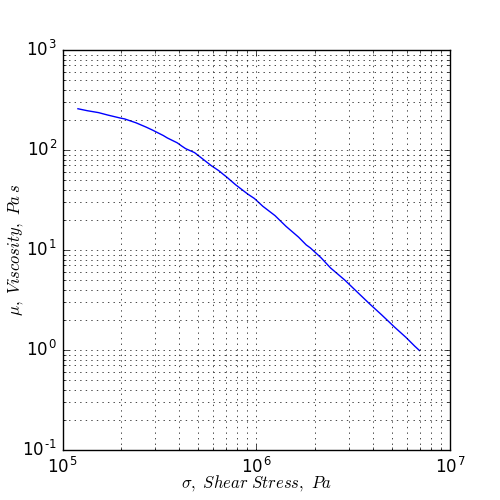
\includegraphics[scale=0.5]{figures/fig_shear_behav_thin.png}
			\caption{Shear Thinning}
			\label{figshearthin}
			\footnotesize 
			Viscosity vs. shear stress for a shear-thinning fluid. Glass spheres 15 $\mu$m in diameter suspended in thermoplastic.
			%Better Graph? Talk more about the parts of the graph. Newtonian area at low shear, non-Newtonian at high
		\end{subfigure}
		\begin{subfigure}[t]{0.45\textwidth}
			\centering
			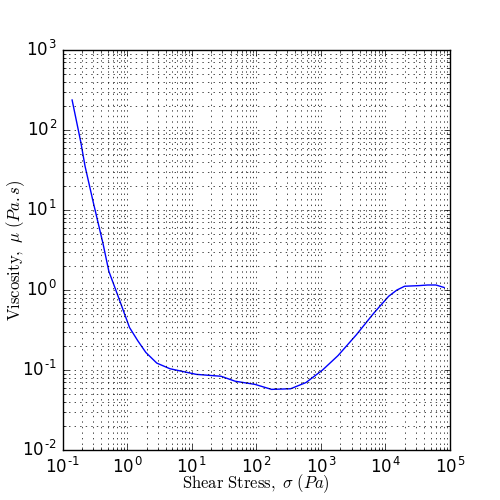
\includegraphics[scale=0.5]{figures/fig_shear_behav_thick.png}
			\caption{Shear Thickening}
			\label{figshearthick}
			\footnotesize 
			Viscosity vs. Shear stress for a shear thickening fluid ($\phi=0.5$, colloidal latex particles dispersed in water). The initial shear thinning region can be seen before the fluid acts Newtonian until the shear stress reaches a critical yield stress and the fluid appears to thicken. At high stress, the fluid once again acts Newtonian.
		\end{subfigure}
		\label{figshearthinthick}
		\caption{Non-Newtonian Behaviour: Viscosity vs Shear Stress (adapted from \cite{figshearthin, figshearthick})}
	\end{figure}
	
	\noindent
	Viscosity is measured in the lab using a rheometer. There are three general types of rheometers: capillary, cone-and-plate, and rotational. Capillary rheometers consist of a tube of known cross section, through which the test fluid is forced (by pumping, by piston). The viscosity can be found by measuring the flow rate and pressure gradient, and using the Hagen-Poiseulle equation for laminar flow through a pipe \cite{backcaprheom}. Cone-and-plate rheometers consist of a cone rotating in fluid on a stationary plate. The torque required to spin the cone at a speed is measured. The shear stress in the fluid is proportional to the torque output by the motor, and the shear rate is proportional to the rotation rate. %(Information about the CAPR: how does it work, how accurate can it be, what is it usually used for)
	\br
	The rotational rheometer is based upon the idea of Couette flow: two infinitely long plates (separated by a known amount) between which is fluid. As one plate moves, the fluid is sheared. In Couette flow, the strain rate calculation is simplified: strain rate is the first derivative of the velocity of the shear. In Couette flow, the velocity varies linearly with accross the gap therefore the strain rate is constant. A Couette cell is a practical approximation of the infinitely long plate shear scenario. The cell is constructed from two cylinders: the outer cylinder and the inner cylinder. The cylinders are positioned vertically close together to limit the amount of fluid shearing on the bottom of the inner cylinder. This set up mimics the couette flow idea and closely replicates the effect, resulting in linear variation of velocity, and a constant strain rate \cite{couetteshearcell}.
	
	\section*{Colloidal Suspensions and Jamming} % last edited 8/3/2017
	Fluids consisting of solid particles suspended in a liquid are prone to non-Newtonian behaviour, most commonly shear thinning. Some suspensions exhibit shear thickening behaviour. The concept of hydroclustering has been used to explain this shear thickening behaviour: as the suspension undergoes shear, the particles are forced together forming larger particle groups. This increases the effective viscosity compared to low shear flow where the particles movements are not as restricted \cite{figshearthick}. The order-disorder transition  theory explains the increase in viscosity as being due to an increase in stress causing the particles to become disordered. Initially there is a drop in viscosity, due to the particles in the suspension becoming more ordered. Then, as the stress is increased past a yield stress, the viscosity begins to increase due to a disruption in the order of the particles \cite{backbrownjaegrev}. % other theories?
	\br
	Shear thickening can be split further into continuous shear thickening (CST) and discontinuous shear thickening (DST). In CST the viscosity increases proportionally to shear after a yield stress. However, with DST the viscosity suddenly (almost asymptotically) jumps upwards. DST has been associated with an apparent decrease in volume fraction of suspensions - hence its alternative name of dilatency. This effect also supports the order-disorder-transition theory of shear thickening: you would expect the volume fraction to decrease (void fraction to increase) if the particles are going from a neat, ordered arrangement into extreme disorder \cite{backbrownjaegrev}. 
	\br
	DST is linked to the concept of jamming, which is \textit{"the conversion of a liquid system into a solid by imposed stress"} \cite{backhawjam}. Jamming is found in many different systems: in solids entering a hopper \cite{back2djam}, in pedestrians walking down a corridor \cite{backpedjam}, and in traffic \cite{backcarjam}. This can cause problems in processes: halting flow, damaging mixing equipment \cite{backshearjambertrand}. \br 
	%Volume fraction of the suspension mixture is an important property when looking at jamming. A suspension's volume fraction (\( \Phi \)) is the ratio of the volume of suspended particles to the volume of fluid in the suspension. For spherical particles, there is a maximum fraction. The closest packing that can occur (face-centred cubic) results in a particle volume fraction of \( \Phi = 0.74 \). However, at this packing the suspension is no longer a suspension and the particles are all in constant contact. The highest volume fraction of a suspension that still allows fluid to pass between the particles (particles are lubricated) is \( \Phi = 0.64 \) \cite{backguypoonjam}. As volume fraction increases, the likelihood of a suspension to undergo jamming increases. 
	%\br
	%The equivalence of particles to hard spheres is an approximation of the physical properties of the particles in a suspension. A "hard sphere" particle is a particle which is roughly spherical and with a fixed (non-intersectable) volume. \cbh 
	%\br
	An interesting phenomenon that occurs in jamming suspensions is the formation and dissipation of "cracks" on the surface of the suspension. This can be directly seen in Figure \ref{cforscracks}. The cracks have been associated with a localized change in volume faction of the suspended particles \cite{backhawjam}. Another interesting optical property of jammed suspensions: the surface of a shear suspension has been found to alter texture, evidence of "dilation" \cite{backbrownjaegrev}: caused by the particles in shear attempting to move around each other but having to take an inefficient route therefore decreasing the volume fraction of the suspension. This draws more fluid into the bulk and then the surface appears rough in texture, as opposed to glossy. 
	\begin{figure}[!htb]
		\centering
		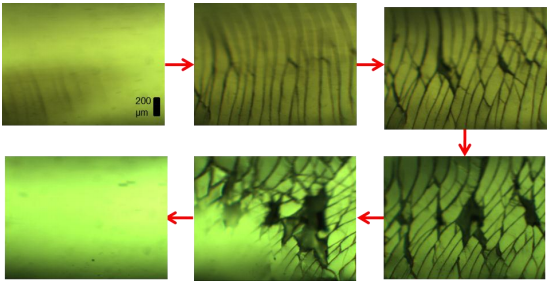
\includegraphics[scale=0.4]{images/cfors_cracks.png}
		\caption{Suspension Surface Cracks (taken from \cite{thescforsyth})}
		\label{cforscracks}
	\end{figure}
	\section*{Raspberry Pi}
	It was noticed that people were not properly learning about how computers work in schools and universities and so a team of academics at the University of Cambridge created the Raspberry Pi Foundation, and developed the Raspberry Pi Model A as a platform to facilitate education \cite{pihistory}. The Raspberry Pi is a small (85mm x 56mm \cite{pi3mechdraw}) computer. By default, it runs a version of GNU/Linux called "Raspian". There are a number of alternative operating systems suitable for different applications (media center, embedded smart technology) \cite{piotheros}.  \newline
	\begin{figure}[!htb]
		\centering
		\includegraphics[scale=0.3]{images/annotpidia.png} %https://www.draw.io/#Hcbosoft%2Fpi_rheo_proj%2Fmaster%2Fwrite_up%2Fimages%2Fannot_pi_dia.xml
		\caption{Raspberry Pi 3 Model B (adapted from  \cite{pi3info})}
		\label{pidia}
	\end{figure} \newline% \noindent
	The first Raspberry Pi (Model A) had a single core 700MHz processor and 256MB of RAM \cite{pi1info}, while the current Raspberry Pi 3 Model B has a quad core 1.2GHz and 1GB of RAM (also including built in WiFi and Bluetooth) \cite{pi3info}. 
	\br
	Despite being initially designed for educational purposes, the Raspberry Pi has found success in other areas such as with hobbyists \cite{pihobbynotedu} and in industry \cite{pimorethanedu}. As a research tool, the Raspberry Pi has been used as a miniature server for researching the traffic patterns in data centres (the Pis were emulating the behaviours of full scale servers) \cite{piglasgowdc}.
	\br
	What makes the Raspberry Pi attractive as a process controller are the GPIO pins (General Purpose Input/Output, see Figure \ref{pidia}) made available on the main board, similar to a microcontroller. These pins allow electronic circuits to interface with the Raspberry Pi, and thus software to interact with the real world in a way that is not easy to accomplish with a traditional computer. This marriage of microcontroller and desktop computer allows for development, and testing in a single package. In addition, the Raspberry Pi retails (at the time of writing) for \pounds 30.00 \cite{picost}, making it a very cost effective alternative to other control solutions (which can cost several hundred pounds \cite{otherpcucost}). 
	\br
	The GPIO pins are the heart of the Raspberry Pi. Each pin is numbered so that they can be referenced and distinguished between their functions. Some of the pins on the GPIO header are power pins, some are grounded, most are GPIO pins. Each GPIO pin supports digital signals. Resistors attached to the GPIO pins can be used to "pull-up" or "pull-down" the signal. If a pin is pulled down, its signal is normally low - it needs to be actively raised high. If a signal is pulled up, it is normally high - it can be lowered by connecting it to ground, but without that it will try to be high. These pull-up and pull-down resistors are included in the Raspberry Pi internally and are activated/deactivated programmatically.
	
	\begin{figure}[!htb]
		\centering
		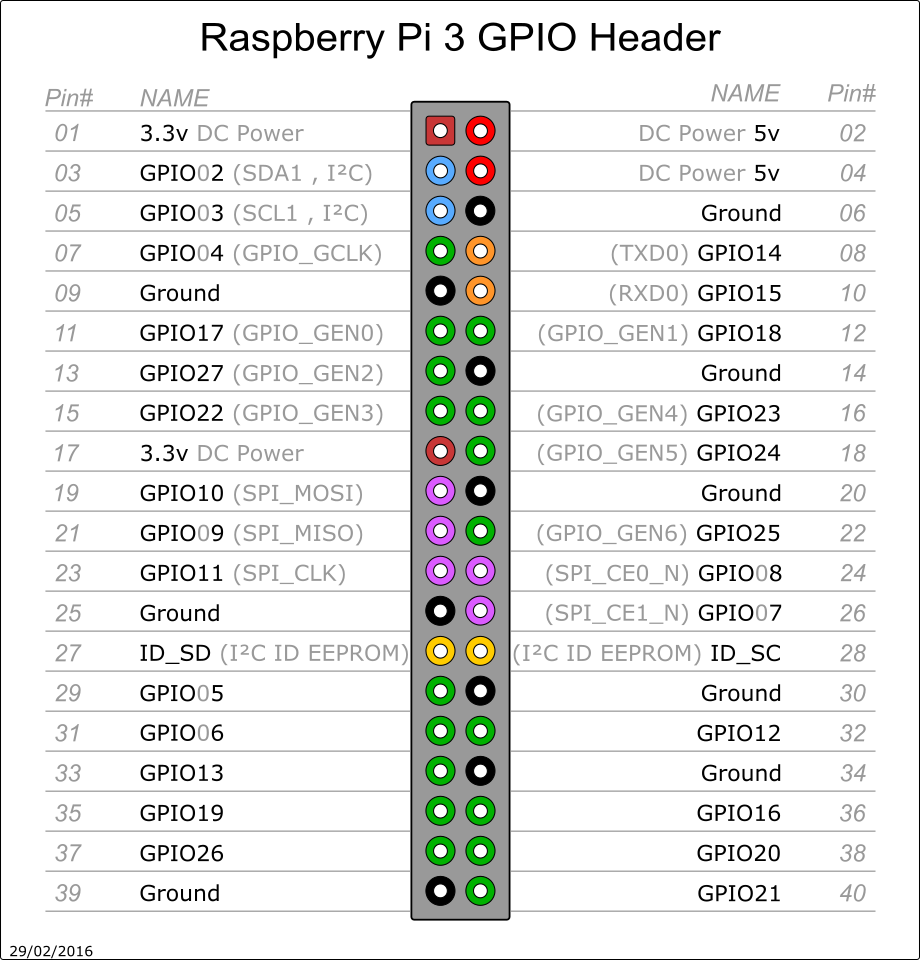
\includegraphics[scale=0.2]{images/gpiopinout.png}
		\caption{Raspberry Pi 3 Model B GPIO Pinout Diagram (taken from  \cite{pigpiopinout})}
		\label{gpiopinout}
	\end{figure}
	
	\noindent
	In addition to simple GPIO functionality, some of the Raspberry Pi's GPIO pins have special functionality, like the ability to use serial communication making inter-device communication much easier. To send the number 1750 to an integrated circuit, the Raspberry Pi would need at least 11 free GPIO pins. While this is not impossible, the number of GPIO pins used for this single action is inconvenient. This can easily be sent via serial connection with just two wires. There are several serial communication options built into the Raspberry Pi: $I^2C$ (Inter-Integrated Circuit) and SPI (Serial Peripheral Interface) are two. SPI uses up to four wires for communication: a clock line for synchronising data transfer, a master-out-slave-in data line (MOSI), a master-in-slave-out (MISO), %not the soup
	and a chip select line for selecting which slave device the master is communicating with.
	%\br
	%Pins 3 and 5 can also be used to communicate with integrated circuits with the \(I^2 C\) protocol (Inter-Integrated Circuit). This allows bytes of data to be sent over only two wires \cite{backwhatisi2c}. This is done by \textit{serial communication}. Serial communication is where each bit of data (starting with the most significant bit, the highest value bit) is sent one after the other down a wire (the "data" line) \cite{backwhatisserpar} while another wire is used to synchronise the communication beteween devices (the "clock" line). Pins 19, 21, 23, 24, and 26 are used for another serial communications protocol, the Serial Peripherial Interface (SPI) protocol \cite{backwhatisspi}. SPI is similar to \(I^2 C\), although it differs in a few key ways.  \(I^2 C\) manages sub devices on the network using an address system which enables anything up to 128 devices connected together in one go, however SPI uses a simple select system where a signal is sent from a GPIO to the SPI device to tell it to expect instruction. This makes the SPI device far easier to work with, but less useful as the number of daisy-chained devices is limited by the number of free GPIO pins. 
	%\br
	%The high level languages used to create programs on desktop computers can be similarly used to write software on the Raspberry Pi. There are a number of software packages available for facilitating the communication with the GPIO pins. Built in to the Raspberry Pi are some basic packages, but for greater functionality third-party libraries are available for anyone to download and use\cite{pilibswiringpi, pilibspigpio}. The programming language "Python" is popular among software developers. Python is a high level, object oriented, interpreted language; making it well suited to quickly develop clean and easy to use software. Due to its popularity, Python has a vast number of packages available to perform any number of functions.

%=====------++++++=====------++++++=====------++++++=====------++++++=====------++++++=====------++++++=====------++++++=====------++++++=====------++++++=====------++++++=====------++++++=====------++++++=====------++++++=====------++++++=====------++++++=====------++++++
	% \nc{Description of the Organisation}
	% Paragraph on what strathcyde is here
	
	\nc{Description of the Work}
	%Elaborate on issues mentioned in introduction. Use a logical development, not necessarily in chronological order. Explain the significance, purpose and nature of your work. Describe methods used and outcomes. Try to ensure a balanced treatment of issues, in accordance with their relative importance, and excluding irrelevant material. Present results and discuss around them. Explain the significance of these results and their impact on the organisation. Comment on technical difficulties you may have experienced. In a long report, subdivide with appropriate sub-headings, or divide this section into different sections. Equations should be numbered sequentially.
	
	% TODO :: 
	% UNCERTAINTIES IN MEASUREMENTS
	% PHOTOGRAPH OF SET UP (IN PROGRESS)



	\section{Hardware Setup} % last edited 7/3/2017
	The experiment is based around a Couette cell consisting of two concentric cylinders with a fluid in between. The inner cylinder can be rotated by a DC motor (model 970D161) while the outer cylinder is fixed. The motor is controlled by a Raspberry Pi, which sets the rotational speed and reads the torque load on the motor. This is used to calculate the viscosity of the fluid. Motor speed is read in using a secondary motor acting as a dynamo. The dynamo is spun by the inner cylinder motor and produces a voltage proportional to its rotational speed. This voltage is then read in by the \rpi.
	Figure \ref{expdia} gives a diagram of the set-up, dimensions of the couette cell are summarised in Table \ref{tabcellgeom}.\newline
	\begin{figure}[!htb]
		\centering
		\includegraphics[scale=0.3]{images/exp_set_up.png} % https://www.draw.io/#Hcbosoft%2Fpi_rheo_proj%2Fmaster%2Fwrite_up%2Fimages%2Fexp_set_up.xml
		\caption{Diagram of the Experimental Apparatus}
		\label{expdia}
	\end{figure} \newline \noindent
	\begin{table}
		\centering
		\begin{tabular}{|c|c|}
			\hline
			Reading 						& Value ($mm$) \\
			\hline
			Inner Cylinder, Diameter 		& $30.512 \pm 0.590 \%$\\
			Inner Cyliner, Height 			& $46.795 \pm 0.577 \%$\\
			Outer Cylinder, Inner Diameter 	& $39.111 \pm 1.23 \%$\\
			Outer Cylinder, Outer Diameter 	& $44.151 \pm 0.476 \%$\\
			Outer Cyliner, Height 			& $39.753 \pm 1.41 \%$\\
			\hline
		\end{tabular}
		\caption{Couette Cell Geometry}
		\label{tabcellgeom}
	\end{table}
	\br
	The outer cylinder is made of glass and is attached to a metal base with epoxy so that it can be easily clamped in position. The inner cylinder is a perspex cylinder built onto the shaft of the motor. The motor, holding the inner cylinder, is held in place by a clamp stand. This clamp stand also holds the dynamo in position.\br
	The electronic circuits were built onto a breadboard, which allowed for quick alterations to be made to the circuitry during development, with requiring soldering. Wires connect the electronics to the motor, dynamo, and the power source. A ribbon cable connects the full 40 GPIO pins from the Raspberry Pi to the breadboard circuitry.
	
	\section{Electronic Circuits} % last edited 21/3/2017
	%in depth description of relevant electronic circuits
	Figure \ref{circfull} is a schematic of the entire electronic circuit. The circuit can be split into two sections: the first consists of an analogue to digital converter and the sensor components, and the second consists of the potentiometer and various driver components required to set the motor's supply voltage.
	\begin{figure}[!htb]
		\centering
		\includegraphics[scale=0.3]{images/circfull.png}
		%https://www.draw.io/#Hcbosoft%2Fpi_rheo_proj%2Fmaster%2Fwrite_up%2Fimages%2Fcircfull.xml
		\caption{Schematic Diagram of Electronic Circuits}
		\label{circfull}
	\end{figure}

	\subsection*{\textit{Sensor Input}} % last edited 21/3/2017
	%Dynamo
	The speed of the motor was gauged using a second motor acting as a dynamo. The dynamo motor was linked to the first motor by a belt and pulley system. The dynamo motor produces a voltage proportional to the speed it is spun at. This sensor therefore provides a qualitative indication of the speed. A pulley was attached to the dynamo, and a rubber belt was used to transfer rotation from the inner cylinder of the Couette cell to the dynamo. The output from the dynamo was fed into an ADC (MCP3008). The ADC works by comparing an input voltage to a reference voltage. Here, the reference voltage was a 3.3V line direct from the Raspberry Pi. This was chosen as it is regulated by the Raspberry Pi and should remain constant thus limiting error in the ADC measurements. The output signal from the ADC is a number between 0 and 1023 (a 10-bit binary number) scaled depending on the input voltage and the reference voltage, and rounded to the nearest integer. See Equation \ref{eqnadc}.
	
	\begin{equation}
		S_{10} \approx 1023 * \frac{V_{in}}{V_{ref}}
		\label{eqnadc}
	\end{equation}
	
	\nomenclature{$S_{10}$}{ADC 10 bit output signal\hfill --}
	\nomenclature[aV  ]{$V_{in}$}{ADC input voltage\hfill $V$}
	\nomenclature[aV  ]{$V_{ref}$}{ADC reference voltage\hfill $V$}
	
	\noindent
	The dynamo speed sensor was the final choice after two other methods were attempted. A Hall effect sensor was used to detect the presence of a magnet attached to the inner cylinder. This was set up such that the Raspberry Pi could (via the HES) calculate the number of rotations in a given time period, or measure the length of time in the gap between rotations. A similar method used a light gate (a UV LED and a phototransistor) and a mask attached to the inner cylinder. As the cylinder rotates, the mask blocks the UV light from shining on the phototransistor and thus the transistor blocks the flow of electrons between its gate and source pins - which can be detected by the Raspberry Pi. Issues arose, however, with the Rapsberry Pi's ability to measure time accurately. In addition, the python environment is not well suited to accurately reporting time due to the memory management processes enacted by python and even the underlying linux kernel in the operating system \cite{backrpibadrealtime}. This lead to the dynamo qualitative speed sensor to be used in favour of the quantitative speed sensors due to its ease of use and reliability.
	\br
	To sense the current drawn by the motor, a Hall Effect Current Sensor, or HECS (ACS712, 30A sensing range) is used. A Hall effect sensor produces a voltage proportional to the strength of a magnetic field which is produced by running a current through a coil with a magnetically permeable core. The sensor package contains both the coil and the hall effect sensor such that when a current is passed between the sensor pins, a voltage proportional to this current is produced accross the output pins.. The normal output (at zero amps sensed) is half of the supply voltage of 5V. The direction of the current will determine whether the voltage will increase above 2.5V or decrease below 5V. The current draw by the motor will only ever be in a single direction, so the directional information is unnecessary. Due to the large possible range of the device (being able to sense from -30A to +30A), the voltage will be boosted to allow the ADC to see a better range of values. In addition, the direction information is removed by subtracting 2.5v. The singal is then amplified by 10 and fed into the ADC (channel \#1). 
	\br
	To reduce noise in the HECS reading, a further two sensors (both ACS712s, 5A sensing range) were used together with the original sensor. The second and third sensors had a smaller sensing range, which was better suited to this application and they did not require boosting to improve the resolution of the signal. The data from the three sensors is averaged together in data processing to provide a more reliable signal.

	\subsection*{\textit{Motor Speed Control}} % last edited 21/3/2017
	The speed of the motor is controlled by altering the supply voltage to the motor. A higher supply voltage, a higher rotational speed. The Raspberry Pi sends a digital serial signal (using the SPI protocol) to a digital potentiometer (MCP4131) which then sets its wiper resistance accordingly. The potentiometer is part of a voltage divider, the output voltage of which varies with the potentiometers resistance and therefore can be controlled by the Raspberry Pi.\br
	Within the potentiometer: \(R_{AW}\) is the resistance between terminal A and the wiper pin, and \(R_{WB}\) is the resistance between the wiper and terminal B. The data sent to the potentiometer determines the values of \(R_{AW}\) and \(R_{WB}\), which will total a constant value: \(R_{pot} = 10\ k\Omega \). The digital potentiometer is used in a voltage divider configuration, which allows the voltage in a parallel circuit to be controlled. When the resistance is changed to a new value, the voltage across the motor will change according to Equation \ref{eqnvoldiv}. Resistor \(R_2\) is used to set the minimum output voltage. At \(R_2 = 0\ \Omega\), the output would vary between 0v and 5v. While this would also be useful, it limits the resolution of the potentiometer as the bottom volt of this range will not be able to sufficiently power the motor. To bring this minimum up (and thus be able to utilise more of the potentiometer) \(R_2\) is set at \(3\ k\Omega \). The digital potentiometer can only handle voltages up to 5v across its terminals, an amplifier (gain = 2.1) is used to boost the voltage range from 1.2v to 5v up to 2.52v to 10.5v. A transistor (BD243C) is used to boost the current output from the amplifier, which can only supply around 20mA. The transistor boosts this up to 2A (hFE = 100).
	\begin{equation}
		V_{out} = V_{in}\times \frac{R_2 + R_{WB}}{R_2 + R_{pot}}
		\label{eqnvoldiv}
	\end{equation}
	\begin{equation}
		V_{min} = V_{in}\times \frac{R_2}{R_2 + R_{pot}}
		\label{eqnminvol}
	\end{equation}
	\begin{equation}
		V_{max} = V_{in}\times \frac{R_2 + R_{pot}}{R_2 + R_{pot}} = V_{in}
		\label{eqnmaxvol}
	\end{equation}
	
	\nomenclature[aV ]{$V_{out}$}{Voltage output \hfill $V$}
	\nomenclature[aV ]{$V_{in}$}{Voltage input \hfill $V$}
	\nomenclature{$R_{AW}$}{Resistance between potentiometer wiper and A terminal\hfill $\Omega$}
	\nomenclature{$R_{WB}$}{Resistance between potentiometer terminal B and wiper\hfill $\Omega$}
	\nomenclature{$R_{pot}$}{Resistance between terminals A and B on the potentiometer\hfill $\Omega$}
	\nomenclature{$R_{AW}$}{Resistance value ofthe resistor between B terminal on the potentiometer and ground\hfill $\Omega$}
	
	\noindent
	The Raspberry Pi sets the motor speed by setting the resistance in the digital potentiometer. The Pi sends a 7-bit digital signal to the pot, indicating the resistance desired. Within the potentiometer is a network of resistors, and this number will determine the path taken through the circuit, the higher the number, the higher \(R_{WB}\) will be. When this increases, the voltage across the bottom resistor will decrease and the voltage across the motor will mirror this.\br
	A 7-bit number has a maximum value of 127 ($2^7 - 1 = 127$). Therefore the potentiometer terminal B-wiper resistance will increase by $78.7 \Omega$ given a unit increment in potentiometer value (Equation \ref{eqnpotres}). Combining this with Equation \ref{eqnvoldiv} gives an equation for motor supply voltage (also knowing the gain of the operational amplifier circuit) - Equation \ref{eqnmotsupvol}.
	
	\begin{equation}
	V_{wiper} = V_{AB}\times \frac{3k\Omega + \left(78.7\Omega \times pv\right)}{13k\Omega}
	\label{eqnpotres}
	\end{equation}
	
	\nomenclature[aV ]{$V_{wiper}$}{Voltage level at the digital potentiometer output \hfill $V$}
	\nomenclature[aV ]{$V_{AB}$}{Voltage accross the potentiometer terminals\hfill $V$}
	
	\begin{equation}
	V_{ms} = 0.0636V \times pv + 2.423V
	\label{eqnmotsupvol}
	\end{equation}
	
	\nomenclature[aV ]{$V_{ms}$}{Motor supply voltage\hfill $V$}

	\section{Software}
	The Raspberry Pi runs a version of GNU/Linux called "Raspbian" - specially developed for the Raspberry Pi's ARM Processor. Raspbian is a desktop operating system, and can perform all of the tasks a full size computer can (text processing, internet browsing, etc.). This presents one of the main features of the Raspberry Pi - it can be both development station and testbed. Software was written to enable the Raspberry Pi to communicate with the hardware using the Python language. Python was chosen as it is a very popular, easy to use, and easy to read language (there are rules about how python should be properly written in order to maintain easy-to-read code \cite{pep8ref}). Its popularity means that there is an abundance of software packages available for inclusion. 
	\br
	Packages used here:
	\begin{itemize}
		\item \texttt{RPi.GPIO}\cite{citerpigpio}: comes pre-installed on Raspian and was used for accessing the GPIO pins from a Python environment.
		\item \texttt{spidev} \cite{srcspidev}: used to communicate with devices in an electric circuit using the Serial Peripheral Interface (SPI) protocol.
		\item \texttt{numpy} \cite{numpyref}: used to perform calculations efficiently in the python environment and to fit equations to empirical data (using the \texttt{numpy.polyfit} function).
		\item \texttt{scipy} \cite{scipyref}: used to perform scientific manipulations of data. Primarily used in this project to filter data using functions from the \texttt{scipy.optimise} package.
		\item \texttt{pandas} \cite{pandasref}: used to read Comma Separated Value (\texttt{.CSV}) files - the file format used to log data from experiments.
	\end{itemize}
	
	\begin{figure}[!htb]
		\centering
		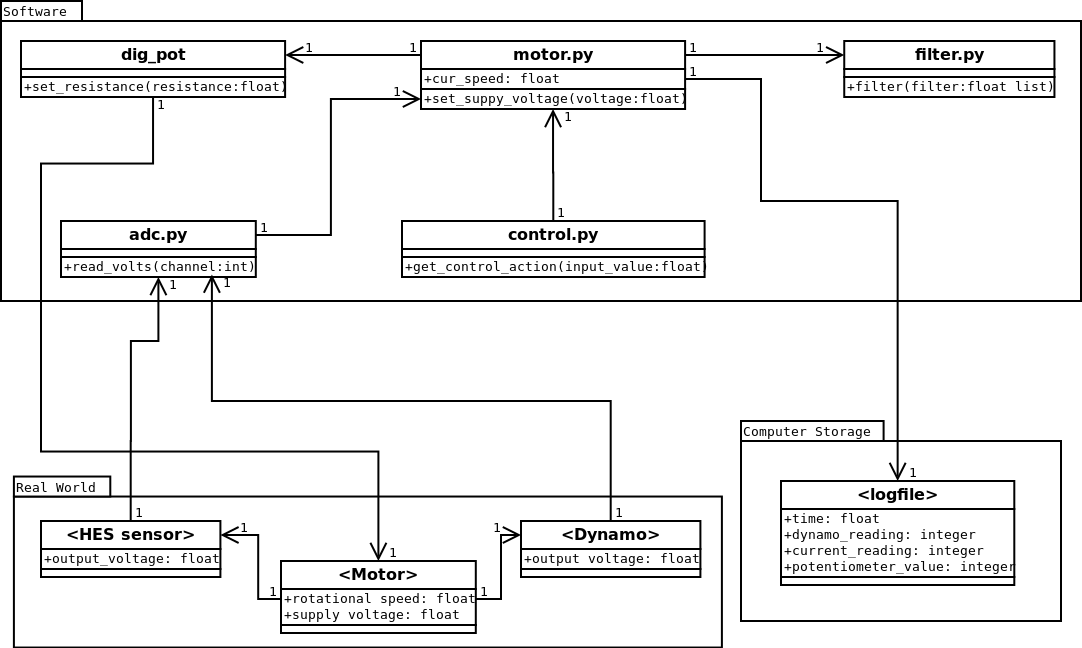
\includegraphics[scale=0.35]{images/codemap.png}
		%RE DO, SOFTWARE WAS SHUFFLED A BIT?
		\caption{Class Diagram}
		\label{figcladia}
	\end{figure}
	
	\noindent
	The software is organised into different classes (see Figure \ref{figcladia}):
	\begin{itemize}
		\item Digital Potentiometer \newline 
		This class manages the sending of data to a digital potentiometer and keeps a record of some key data.
		\item ADC \newline 
		This class manages the sending and receiving of data between the Raspberry Pi and the ADC.
		\item Control\newline 
		This class is a discrete time implementation of the PID algorithm used in process control.
		\item Motor \newline
		This class makes use of the digital potentiometer class to control the voltage supplied to the motor, the ADC class to read in the speed of the motor and the current drawn by the motor. This data is logged at a set rate to be used in calculating the viscosity.
		\item Noise Filter \newline
		A collection of functions that can be used to reduce noise in read data.
	\end{itemize}
	Full copies of the software source code can be found in Appendix 1.
	
	\subsection*{Digital Potentiometer} % last edited 13/3/2017
	This class enables the software to interact with the digital potentiometer (model MCP4131) using the SPI protocol. This class makes use of the \texttt{spidev} package to enable SPI communication. The class contains a function to set a value on the resistor (as an integer number between 0 and 127), and is set up such that multiple digital potentiometers can be included on the same circuit.
	\br
	The class is used, as with all normal classes, by first creating an instance of a class object, passing along the initialisation parameters. These parameters are set in the source code as the parameters to the "\texttt{\_\_init\_\_}" function. For this class, there is only one initialisation parameter: "\texttt{chip\_select}", an optional parameter which tells the spidev package which SPI device to talk to. This parameter is 0 by default, but can be changed if the class is used in a different instance to manage another digital potentiometer.
	\br
	To set the potentiometer resistance, a value between 0 and 127 (inclusive) is sent to the potentiometer using the "\texttt{set\_resistance}" function. This function only requires one parameter - the value to be sent. The spidev package is used to send this value to the correct register on the potentiometer, causing it to alter its resistance.
	
	\subsection*{ADC} % last edited 13/3/2017
	The ADC class enables the software to interact with the analogue to digital converter (both model MCP3008) via the SPI protocol. As with the digital potentiometer, this class makes use of the spidev package. \br
	The initialisation function for the ADC class has two parameters, both optional. The first is a chip select parameter (used to tell spidev which device we are trying to communicate with on the SPI network) which has a value of 1 by default. The second parameter is the value of the reference voltage (\texttt{vref}), 3.3 by default, used to calculate the voltage read in by the ADC from the 10-bit value read from the ADC. \br
	Usage of the class is very simple: the "\texttt{read\_data}" function returns the value read from the ADC (a 10-bit number) and takes only 1 parameter (a value from 0 to 7 indicating the channel on the ADC to read from). Further, the "\texttt{read\_volts}" function will read from the ADC and convert the result to a voltage. This function takes a channel indication parameter.
	
	\subsection*{Control} % last edited 13/3/2017
	This class is a discrete-time implementation of a PI controller based upon the PID algorithm (Equation \ref{eqnpidalg}). Due to the random fluctuations in speed caused by the jamming effect, derivative control is not included because derivative action works on the rate of change of the error, therefore a sudden change in the error is going to elicit an extreme response from  the controller which will upset the process. In addition, there will be noise inherent in the signal (discussed in the next section) which will severely impair the controller if derivative action is turned on. 
	
	\begin{equation}
		ca = \pm K_C \left(e + \frac{1}{\tau _I} \int e \space dt + \tau _D \frac{de}{dt}\right)
		\label{eqnpidalg}
	\end{equation}
	
	\nomenclature{$K_C$}{Controller gain}
	\nomenclature[g]{$e$}{Error between the set point and controller input}
	\nomenclature[g]{$\tau_I$}{Integral time constant}
	\nomenclature[g]{$\tau_D$}{Derivative time constant}
	\nomenclature{$K_P$}{Proportional action gain}
	\nomenclature{$K_I$}{Integral action gain}
	\nomenclature{$K_D$}{Derivative action gain}
	
	\noindent
	The control class uses a discrete time transfer function of the controller algorithm, formed by first removing the derivative action and taking a Laplace transform. In Laplace domain notation; $U(s)$ is the controller output, and $e(s)$ is the error between the process output (controlled variable) and the set point. The resulting transfer function is shown as Equation \ref{eqnpitf}.
	
	\begin{equation}
		\frac{ca}{e}(s) = \frac{K_P  s + K_I}{s}
%		\frac{ca}{e}(s) = K_P + \frac{K_I}{s}
		\label{eqnpitf}
	\end{equation}
	
	\noindent
	This class makes use of the \texttt{scipy.signal} package to deal with transfer functions.\br
	The initialisation function for this class has three arguments, described below. Included in the descrption is the data type the function is expecting, and the default value (if applicable).

	\begin{itemize}
		\item \texttt{tuning} - tuple (float, float). Represents the proportional and integral gains respectively.
		\item \texttt{set\_point} - float. Optional. The desired value for the controlled process variable. 0 by default.
		\item \texttt{sample\_time} - float. Optional. The interval time between control action updates. By default, this is automatically calculated, but can be set manually here for simulating the response.
	\end{itemize}

	Function "\texttt{get\_control\_action(Y)}" is used to obtain the control action in response to the input. This function takes a single argument: the process output. Then the \texttt{scipy.signal} package's transfer function class is used to obtain the result from the controller's transfer function, giving a suitable control action.
	\br
	For the controller to be useful, it needs to be tuned. This can be done using a modelled transfer function of the process, such as a First Order Plus Dead-Time (FOPDT) model. Using a model, the controller can be simulated to view how it reacts to different tunings. The class includes a simulation function ("\texttt{do\_sim}") to allow for manual tuning. The function uses a transfer function for the process (a first order model) and simulates process output for a length of time after a step change in set point. The results give an indication of how well the controller can manage the process. 
	\br
	There are a number of techniques used to tune controllers. \cbh

	\subsection*{Noise Filter}
	The data read in by the ADC is noisy - it contains unwanted fluctuations along with the desired signal. Noise can originate from many different sources: mains power supply fluctuations, faults in the conductive materials, fluctuations in temperature and pressure, and even the random nature of electron flow (current)\cite{wileyadvsignproc}. Some noise can be easily predicted and identified (e.g. a 50Hz noise waveform in the signal is probably due to the power supply) but others cannot be so easily predicted. 
	\br
	Filtering techniques can be used to eliminate noise from a signal. Frequency filters remove certain frequencies from the signale. Other filtering techniques include: fitting polynomial equations to sections of the data ("splines") - a more graphical method of removing the noise; using a probabilistic analysis of the data to determine the main response; or using a moving average of the data (which can be weighted to favour the data surrounding the current point being filtered).
	\br
	The filtering algorithm used in the \texttt{filter} function, is a low pass frequency filter using a Butterworth function. Frequency filtering works by moving the signal into the frequency domain by Fourier transform. Then, a function is applied which drops off to zero very quickly - this selects desired frequencies and removes undesired frequencies. Noise in the signal is high frequency, therefore a low pass filter is desired to allow low frequency signals to pass through (the data) and the high frequency signals (noise) to be eliminated.
	
	\begin{figure}[!htb]
		\centering
		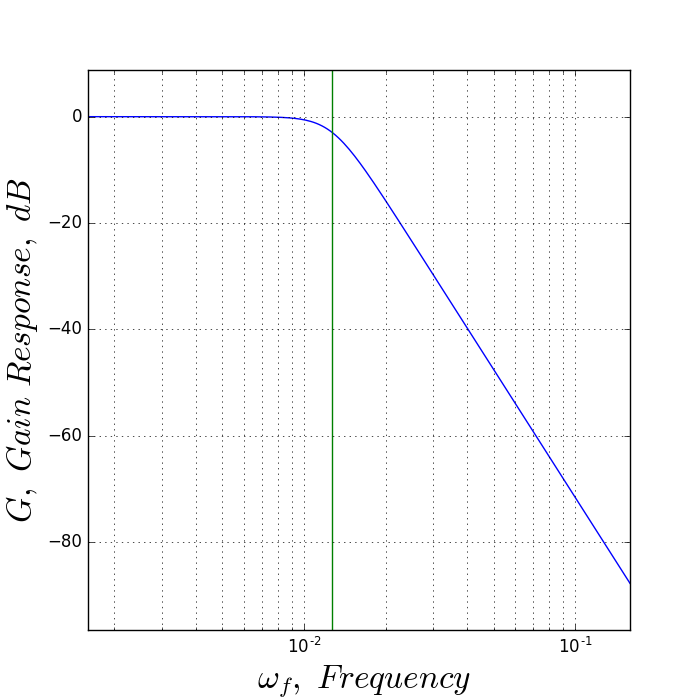
\includegraphics[scale=0.4]{figures/fig_butter.png}
		\caption{Frequency Domain Signal Response To Butterworth Function}
		\label{figbutter}
		\begin{subfigure}{0.8\textwidth}
			\centering
			{\footnotesize 4$^{th}$ order Butterworth filter response (blue line) with 0.0127 Hz cut-off frequency (green line).}
		\end{subfigure}
	\end{figure}
	
	\begin{equation}
		|G(j\omega)| = \frac{1}{\sqrt{1 + \left(\frac{\omega_f}{\omega_{cf}}\right)^{2n}}}
		\label{eqnbuttgain}
	\end{equation}
	
	\nomenclature{$|G(j\omega_f)|$}{Frequence response, or gain\hfill dB}
	\nomenclature{$\omega_f$}{Passed signal frequency\hfill $\pi radians/sample$}
	\nomenclature{$\omega_{cf}$}{Signal cutoff frequency\hfill $\pi radians/sample$}
	
	\noindent
	The Butterworth gain transfer function (Equation \ref{eqnbuttgain}) is applied to the frequency domain signal - responding as in Figure \ref{figbutter}.
	There is a function in the \texttt{scipy.signal} library which creates a Butterworth filter transfer function, and another function which can be used to apply the created filter. This was packaged together in a function ("\texttt{filter.filter()}") within the \texttt{filter.py} package. This function takes in noisy data, applies the filter, and outputs the clean signal. 
	\br
	The butterworth function in scipy has two parameters: \texttt{N} and \texttt{Wn}. \texttt{N} (n in Equation \ref{eqnbuttgain}) is the order of the butterworth function, representing how sharply it removes frequencies above the cut-off frequency. \texttt{Wn} is the cutoff frequency normalised against the signal's Nyquist frequency. The Nyquist frequency is the slowest the sample can be sample without causing issues to arise in the read data (like aliasing: signals appearing to move in one way but actually moving in another, like car wheels in low-framerate videos) and is equal to twice the fastest moving dynamics in the signal. By trial and error, the optimal parameters of the filter function were found to be \texttt{N}$ = 2$ and \texttt{Wn} $ = 0.001$. This represents a butterworth function of order 2 with a cutoff frequency one five-hundredth of the highest frequency data in the signal.
	
	\subsection*{Motor}
	This class uses the ADC class to read in the speed of, and current supplied to motor. The digital potentiometer class is used to control the voltage supply to the motor as well. The overall goal of the motor class is to manage every aspect of the motor, and to record as much relevant data as possible. 
	\br
	The class is initialised with several optional variables; most are used by the motor class itself while some are for setting up the ADC class, and some are for setting up the digital potentiometer.
	\br
	Motor-relevant arguments:
	\begin{itemize}
		\item \texttt{startnow} - a boolean value indicating whether the speed poll thread should begin when the class is first instantiated. \texttt{False} by default.
		\item \texttt{poll\_logging} - a boolean value indicating whether data should be logged by the motor to file. \texttt{True} by default.
		\item \texttt{log\_note} - a string added to the log file to give more information about the logged data (the test conditions etc). \texttt{"DATETIME"} by default, replaced by the current date and time when the log is written.
		\item \texttt{log\_titles} - a list of strings giving the headings to be included above the data in the log.
		\item \texttt{log\_dir} - string, path to directory where the logged data will be saved.
		\item \texttt{i\_poll\_rate} - "inverse poll rate", the interval between speed polls. A higher value results in sporadic data and lower processing requirements, a low value results in better data but a higher toll on the Raspberry Pi's resources. \texttt{0.1} by default.
		\item \texttt{svf} - "speed-voltage-function", tuple representing the two coefficients in a linear fit equation for the relationship between the motor's rotational speed and the voltage reading in from the dynamo via the ADC. \texttt{(312.806, -159.196)} by default.
	\end{itemize}
	The motor class, once set up, can be used to set the supply to a motor (using a digital potentiometer), can read in the motor's speed and calculate its current draw (using the ADC).
	
	\subsection*{Post Processing and Results}
	Bringing everything together, the rheometry of a fluid can be calculated from the logged data. The motor python class records the time, speed, supply voltage (potentiometer value), and supply current which is used to calculate the torque output from the motor. Knowing the torque and the rotational rate, the shear stress, strain rate, and the viscosity can be calculated. The torque output (\(T\)) from a DC motor can be found using Equation \ref{eqntcomplex} \cite{backdcmotor}. At a load high enough that the motor can no longer spin, the torque output is the stall torque (\(T_s\)). At no load, the speed is at its highest and is called the no-load speed (\(\omega_N\)). By applying these limits to Equation \ref{eqntcomplex}, Equation \ref{eqntlesscomplex} is found.
	\begin{equation}
		T = \frac{k_v V_a}{r_a} - \frac{{{k_v}^2} \omega}{r_a}
		\label{eqntcomplex}
	\end{equation}
	
	\nomenclature{$T$}{Motor torque\hfill $Nm$}
	\nomenclature[g]{$\omega$}{Motor rotational speed\hfill $rad s^{-1}$}
	\nomenclature{$k_v$}{EMF created in motor armature \hfill $N/m$}
	\nomenclature[aV ]{$V_a$}{Motor armature volume\hfill $m^3$}
	\nomenclature{$r_a$}{Motor armature radius\hfill $m$}
	
	\begin{equation}
		T = T_s - \frac{T_s}{\omega_N} \omega = T_s \left(1 - \frac{\omega}{\omega_N}\right)
		\label{eqntlesscomplex}
	\end{equation}
	
	\nomenclature{$T_s$}{Motor stall torque\hfill $Nm$}
	\nomenclature[g]{$\omega_N$}{Motor no-load speed\hfill $rad s^{-1}$}
	
	\noindent
	Where Torque (\(T\), \(T_s\)) is in Nm, speed (\(\omega\) and \(\omega_N\)) is in rad/s. These equations give the torque as a function of the current rotational rate, if the stall torque and no-load speed are known. The no-load speed is a function of the supply voltage and the stall torque was related to the motor's current draw, see later for calibrations and results. \newline
	
	\nomenclature{$v_{NL}$}{Motor rotational speed, no loading\hfill $RPM$}
	\nomenclature{$pv$}{Potentiometer value\hfill }
	
	\noindent
	Combining Equations \ref{eqnsvemp} and \ref{eqntsemp} with Equation \ref{eqntlesscomplex} yields an equation for motor torque as a function of rotational speed and potentiometer value, Equation \ref{eqnmottsvsp}.
	\begin{equation}
		T = \left(0.169\frac{Nm}{A} \times I_{ms} + 0.038Nm\right) \left(1 - \frac{\omega}{0.01138rads^{-1} pv + 0.3844rads^{-1}} \right)
		\label{eqnmottsvsp}
	\end{equation}
	With the torque and the rotational speed known, the next step was to calculate the shear stress and the strain rate.\br
	The strain rate imposed upon the fluid in the gap between the cylinders can be calculated using Equation \ref{eqnavsr}. The strain rate is the derivative of the velocity of the fluid in the gap. If the velocity varies linearly through the gap (as in ideal Couette flow), then the derivative will simply be the velocity ($ms^{-1}$) divided by the gap size ($m$) \cite{couetteshearcell}.
	\begin{equation}
		\dot{\gamma} = \frac{\omega r_i}{r_o - r_i}
		\label{eqnavsr}
	\end{equation}
	
	\nomenclature[g]{$\dot{\gamma}$}{Shear rate\hfill $s^{-1}$}
	\nomenclature{$r_i$}{Inner cylinder radius\hfill $m$}
	\nomenclature{$r_o$}{Outer cylinder radius\hfill $m$}
	
	\noindent
	In a couette cell, shear stress is a force applied over the surface area of the inner cylinder $\left(2\pi r_i L\right)$, and torque is this force multiplied by a distance (inner cylinder radius: \(r_i\)). Therefore shear stress can be calculated from the torque using Equation \ref{eqnstresstorque}.
	\begin{equation}
		\tau = \frac{T}{2\pi{r_i}^2L}
		\label{eqnstresstorque}
	\end{equation}
	
	\nomenclature[g]{$\tau$}{Shear stress\hfill $Nm^{-2}$}
	
	\noindent
	With both shear stress and strain rate known, the viscosity of the fluid can be easily calculated using Newton's Viscosity Law, Equation \ref{eqnvisco}:
	\[\mu = \frac{\tau}{\dot{\gamma}}\]
	
	\section{Empirical Calibrations}
	The design requires that some calibrations are made prior to use. The method, and results of each calibration are included in this section.
	
	\subsection*{Dynamo Calibration}
	The goal is to find a function of the dynamo output voltage that gives the rotational rate of the motor (i.e. \(v_m ({V_D})\)). To do this, the motor's speed was varied by varying the supply voltage (using the digital potentiometer) to different discrete levels. The \texttt{motor} class was used to perform this so that sensor readings were logged automatically. At each voltage level, the speed was read several times using a contact tachometer to give the actual speed. The dynamo readings were taken from the logs and filtered using the \texttt{filter} package. The clean dynamo data was then compared to the speed readings taken from the tachometer. The \texttt{numpy} package was used to form a first-order empirical relationship between the variables: Equation \ref{eqnspdvvr}. 
	\br
	The digital potentiometer was to give a supply voltages between 2.275 and 10.723, in steps of 0.528. At each supply voltage, A tachometer was used to read the speed (in m/s). The reading was taken five times per supply voltage and the dynamo voltage level was recorded at intervals of 100ms by the Raspberry Pi. The contact tachometer had to be used carefully, it had to make strong enough contact with the cylinder in order to transfer the speed to the tachometer's rotor, but without impacting the speed of the motor and thus obtain an incorrect reading. The average value of each speed reading, and the dynamo voltage readings were plotted on Figure \ref{figspeedvrvolt}.
	
	\begin{equation}
		v_m = 308.768 \times {V_D} - 167.080
		\label{eqnspdvvr}
	\end{equation}
	
	\nomenclature{$v_m$}{Motor rotational speed\hfill $RPM$}
	\nomenclature[aV ]{$V_D$}{Dynamo output voltage\hfill $V$}
	
	\begin{figure}[!htb]
		\centering
		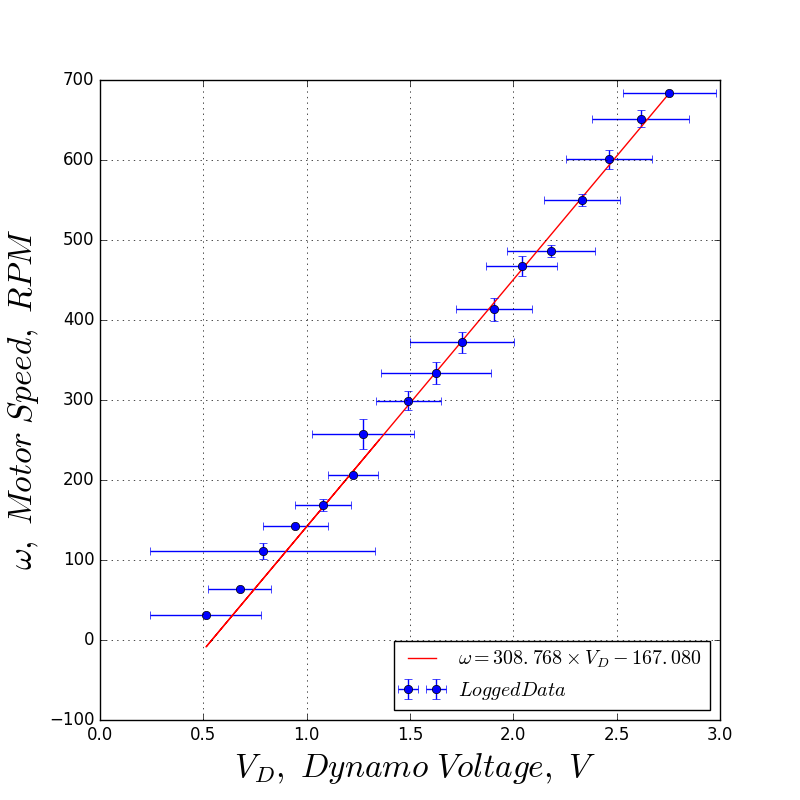
\includegraphics[scale=0.45]{figures/fig_speed_v_rvolt.png}
		\caption{Dynamo Calibration Results}
		\label{figspeedvrvolt}
		\begin{subfigure}{0.9\textwidth}
			\footnotesize Recorded dynamo voltages and corresponding speed in RPM (blue circles). The error bars represent one standard deviation. Also plotted is a line of best fit (red line).
		\end{subfigure}
	\end{figure}
	
	\noindent
	In addition, a relationship between the load-less rotational speed (no-load speed) and the potentiometer value was found, from the same logged data: Equation \ref{eqnsvemp} (see Figure \ref{figdynocheck}).
	
	\begin{equation}
		v_{NL} = 5.13 \times pv + 15.275
		\label{eqnsvemp}
	\end{equation}
	
	
	\subsection*{HES Calibration}
	The goal for this was to find a function of the HES output voltage reading that gives the current drawn by the motor (i.e. \(I_{ms} ({V_{HES}})\)). The current was read at different supply voltages from a multimeter placed in the circuit. The logged data during this run was examined to compare the HES voltage output with the current reading. The current supply was plotted against the HES sensor voltage output (see Figure \ref{figcurevalres}). A first order equation was fit to the data (using the \texttt{numpy} package) to give Equation \ref{eqncurvcr}.
	\begin{equation}
		I_{ms} = 3.580 \times {V_{HES}} - 7.784
		\label{eqncurvcr}
	\end{equation}
	
	\nomenclature{$I_{ms}$}{Motor supply current\hfill $A$}
	\nomenclature{$V_{HES}$}{Hall effect sensor output voltage\hfill $V$}
	
	\noindent
	Where \(I_{ms}\) is the motor supply current, in amps, and \(V_{HES}\) is the voltage output from the Hall Effect Sensor as it enters the ADC, in volts.
	
	\subsection*{Stall Torque}
	The goal of this calibration experiment was to obtain a function of a current drawn by the motor to give the stall torque of the motor. This was obtained by attaching an arm to the motor's shaft and positioning the motor such that the arm hit the top of a balance. The motor was stalled by the presence of the immovable balance, the reading on which will be representative of the force applied by the motor. The stall torque was then easily calculated by multiplying this force by the length of the arm.
	\begin{equation}
		T_s = M_B \times g \times L_A
		\label{eqntscalc}
	\end{equation}
	\begin{equation}
		T_s = 0.1436 \frac{Nm}{A} \times I_{ms} - 0.1391 Nm
		\label{eqntsemp}
	\end{equation}
	
	\nomenclature{$M_B$}{Mass reading on balance\hfill $g$}
	\nomenclature{$L_A$}{Length of arm attached to shaft\hfill $m$}
	\nomenclature{$g$}{Acceleration due to gravity\hfill $ms^{-2}$}
	\nomenclature{$L_a$}{Length of motor shaft arm\hfill $m$}
	\nomenclature{$m_{ba}$}{Mass reading on balance\hfill $kg$}
	
	\noindent
	Mass readings were taken for different supply voltages, the current drawn by the motor was read from an ammeter and recorded along with the mass reading on the balance. Each reading was taken five times per supply voltage and averaged. The results were plotted on Figure \ref{figstalltcal}. An equation was fit to the data; Equation \ref{eqntsemp}.
	
	\begin{figure}[!htb]
		\centering
		\begin{subfigure}{0.45\textwidth}
			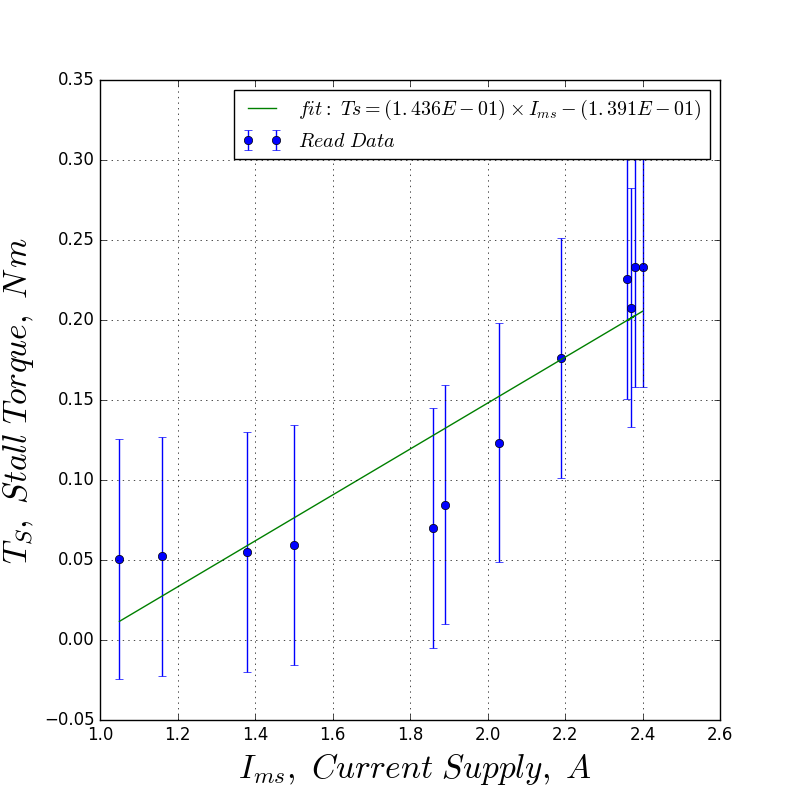
\includegraphics[scale=0.35]{figures/fig_stall_torque_v_supply_current.png}
			\caption{Stall Torque Measurement}
			\label{figstalltcal}
		\end{subfigure}
		\begin{subfigure}{0.45\textwidth}
			\centering
			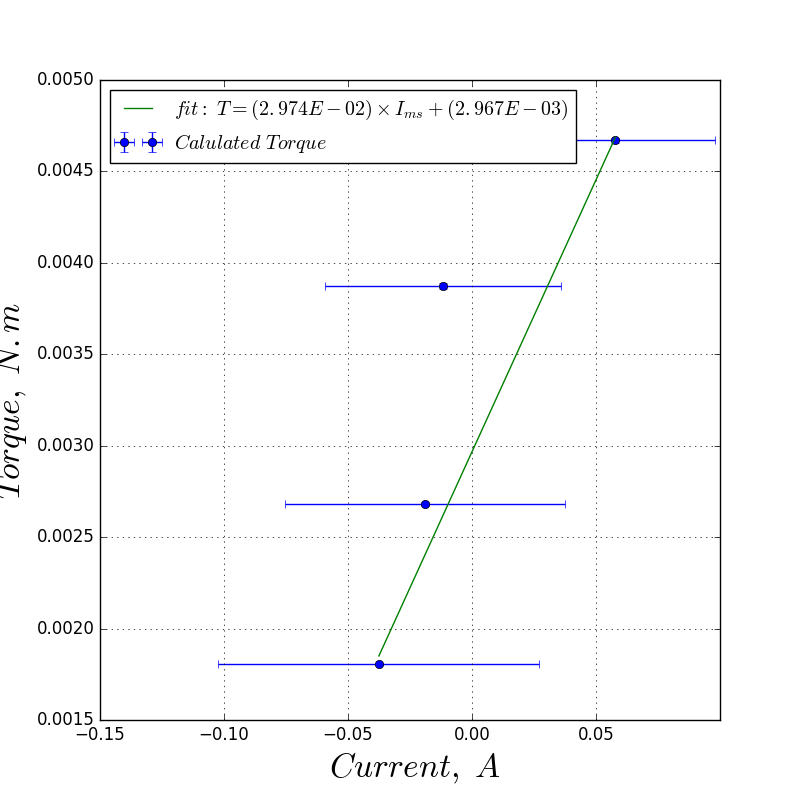
\includegraphics[scale=0.35]{figures/fig_t_ref_cal.png}
			\caption{Torque Calibration}
			\label{figtcal}
		\end{subfigure}
		\caption{Torque Calibration and Measurement Results}
		\footnotesize
		\textbf{(a)} Measured stall torque plotted against supply current (blue circles). 1$^{st}$ order fit equation (green line). Error bars represent 1 standard deviation of the logged data.
		\textbf{(b)} Calibrated motor torque plotted against supply current (blue lines). A first order fit equation is included (green line). Error bars represent 1 standard deviation of the logged data.
	\end{figure}
	
	\subsection*{Torque}
	A relationship between the motor's torque output and the current drawn by the motor was obtained. This was done by putting a fluid of known viscosity into the rheometer and running it at constant shear rate. With the viscosity known and the strain rate known, the shear stress can be calculated. This shear stress was compared with the current draw and a linear equation was fit. \br
	The compositions of the reference solutions were chosen to give solutions of viscosities evenly spaced between 0.001$Pa.s$ ($\mu_{water}$) and 1.141$Pa.s$ ($\mu_{glycerol}$). This was estimated by using tabulated data \cite{seguroberglycsolvisc}. The temperature in the laboratory is roughly 15$^oC$, and so the solutions' viscosity at this temperature was interpolated from data at 10$^oC$ and 20$^oC$. Table \ref{tabreffluvisc} shows both the theoretical and actual viscosities of the solutions used. 30ml of each solution was prepared by measuring out the required volume of glycerol with a syringe (BD Plastic, 5ml) and the required water with a micro-pipette (ErgoOne, 20$\mu l$ to 200$\mu l$) (the pure glycerol solution was far too viscous for the pipette to be able to measure out the volumes accurately). The solutions were split into two containers, one filled up to 20ml to be used in the rheometer, and another filled up to 10ml to be tested separately by a Discovery Hybrid Rheometer 2 (DHR-2). \br
	The DHR-2 was used to obtain an exact value for the viscosity of the solutions used. A small amount of each solution was tested with the DHR-2's 40mm parallel plate head at strain rates from 5$s^{-1}$ to 250$s^{-1}$. each sample was tested 3 times to confirm the result. The theoretically estimated data and the actual viscosity readings differ slightly. This is likely due to water contamination of the glycerol used to produce the solutions. Glycerol is very hydrophillic and will draw moisture out of the air. The viscosity of a glycerol water solution is highly sensitive to the presence of water (increasing water content from 0vol\% to 100vol\% results in the viscosity dropping by 2.3Pa.s) therefore even a tiny amount of water in the glycerol source fluid is going to alter the viscosity hugely. It would be better to use higher viscosity solutions for a better range of values, but the important thing is that the reference solutions are of accurately known viscosity. \newline
		\begin{table}
			\centering
			\begin{tabular}{| c | c | c |}
				\hline
				Composition (vol\% glycerol) & Theoretical Viscosity ($Pa.s$) & Actual Viscosity ($Pa.s$)\\
				\hline
				100.0\% & 2.656 & 1.328 \\
				98.73\% & 2.120 & 1.129 \\
				96.23\% & 1.104 & 0.9061 \\
				93.75\% & 0.613 & 0.6102 \\
				88.87\% & 0.358 & 0.4005 \\
				\hline
			\end{tabular}
			\caption{Compositions and Viscosities of Selected Aqueous Glycerol Solutions at 15$^o C$}
			\label{tabreffluvisc}
		\end{table}
	\noindent
	\newline
	The reference fluids were then ran in the rheometer. Each sample was ran at a constant shear rate (96.9$s^{-1}$). The Raspberry Pi was used to control the settings for each run; the run length and the strain rate were set in a python script. During the run, the supply current and speed of the motor were automatically logged at 1ms intervals, along with the current time and the signal sent to the potentiometer (indicative of the supply voltage to the motor). The torque required to shear the fluid at a shear rate was compared to the increase in motor current draw ($\Delta current$). Average torque requirement for each sample was plotted against the average current draw for each run on Figure \ref{figtcal} and a linear equation was fit, giving an equation for motor torque output with respect to the current draw. This was used to calculate the viscosity of the fluids, with the calibrated calculated viscosity compared to the actual viscosity on Figure \ref{figrheotestres}.

	\section{Evaluation}
	%The project can be split into different sections; design, development, and **evaluation**. In the design phase the overarching goal of the system was decided, including the scope and acceptable limitations. During the development phase prototypes of the system were created and tested against the design specification, altering and improving as necessary. Finally, the evaluation phase saw the use of a completed version of the control system in a rheology experiment, benchmarked against the results of standard lab equipment to gauge the utility of the bespoke apparatus.
	% The varies aspects of the design were tested to evaluate whether they met the design specifications for speed, and accuracy.
	
	\subsection*{Voltage Control}
	To test the efficacy of the voltage control circuit, the voltage was varied (from 2.278V to 10.726V) using the digital potentiometer and measured using a voltmeter. This data was compared with the theoretical result from Equation \ref{eqnmotsupvol} and plotted in Figure \ref{figvoltvval}. This shows the read voltage supply being very close to the theoretically predicted result. A linear equation was fit to the results and compared to the theoretical, again there was excellent agreement. The circuit worked as expected.
	\begin{figure}[!htb]
		\centering
		\begin{subfigure}[t]{0.45\textwidth}
			\centering
			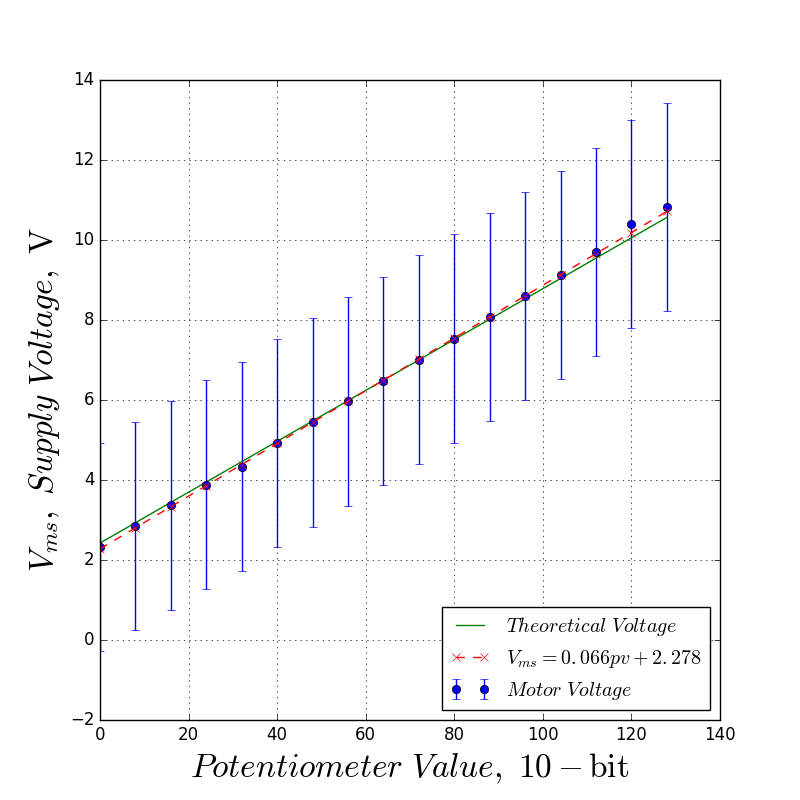
\includegraphics[scale=0.3]{figures/fig_supplyvolt_v_val.png}
			\caption{Voltage Control Check}
			\label{figvoltvval}
			\footnotesize
			Comparison of actual supply voltage (average of three readings) and theoretically expected supply voltage. A linear equation was fit to the read supply voltage data (red dashed line).
		\end{subfigure}
		\begin{subfigure}[t]{0.45\textwidth}
			\centering
			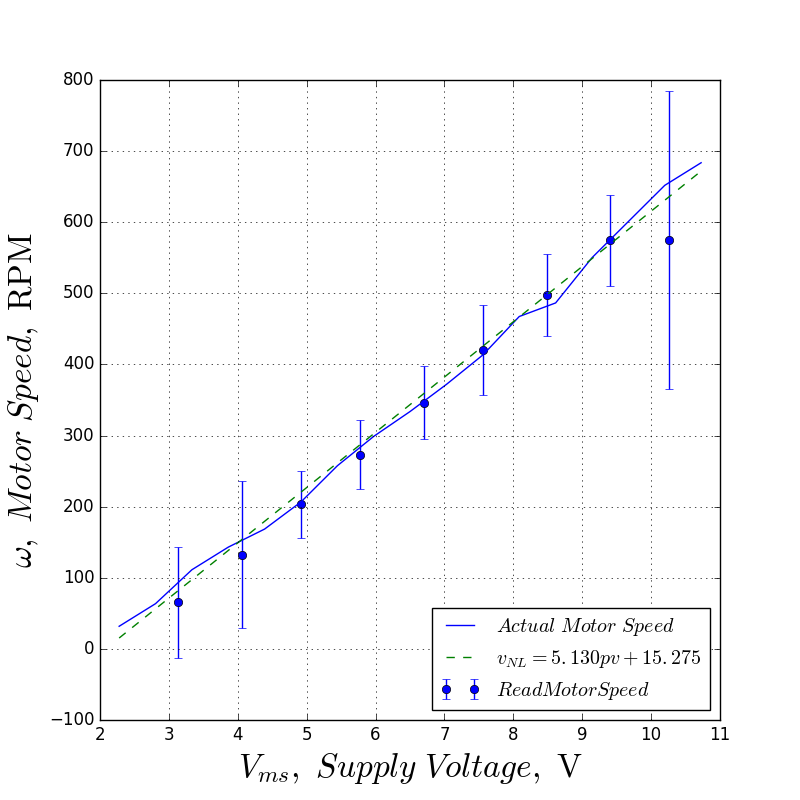
\includegraphics[scale=0.3]{figures/fig_speed_v_val.png}
			\caption{Speed Reading Check}
			\label{figdynocheck}
			\footnotesize
			Comparison of tachometer motor speed readings (blue line), and dynamo speed reading (small red circles). A linear equation was fit to the tachometer readings (dashed green line) and used to calibrate the dynamo sensor.
		\end{subfigure}
		\label{figspeecal}
		\caption{Speed and Voltage Evaluations}
	\end{figure}

	\subsection*{Speed Measurement} % last edited 14/3/2017
	The rotational speed of the motor needed to be measured accurately and quickly, to be able to calculate the viscosity, and to ensure high enough sample rate that the jamming phenomenon can be seen. This was achieved by using a second motor as a dynamo, linked to the controlled motor via a belt. The dynamo will be spun and generate a voltage proportional to the rate at which it is spun, similar to the speedometer in a car. The magnitude of the voltage can be read in using an ADC by the Raspberry Pi (up to 200,000 samples per second). Accuracy of the set-up was tested using a tachometer. The recorded speeds (the tachometer results and the calibrated dynamo results) were plotted on Figure \ref{figdynocheck}. The two signals correspond fairly well, indicating that the speed measurement system works well. However, there was a fairly large amount of noise in the speed measurement signal from the dynamo. This can be seen on Figure \ref{figdynocheck} in the large error bars. The filtering algorithm works well to remove the noise to obtain a useful signal. On Figures \ref{fignoisehistolow} \& \ref{fignoisehistolow}, histograms of the noise at low supply voltage and high supply voltage were plotted respectively. The noise [talk about the shape of the noise (is the histo flat, is it a normal distribution etc etc)]\br
	\begin{figure}[!htb]
		\centering
		\begin{subfigure}{0.45\textwidth}
			\centering
			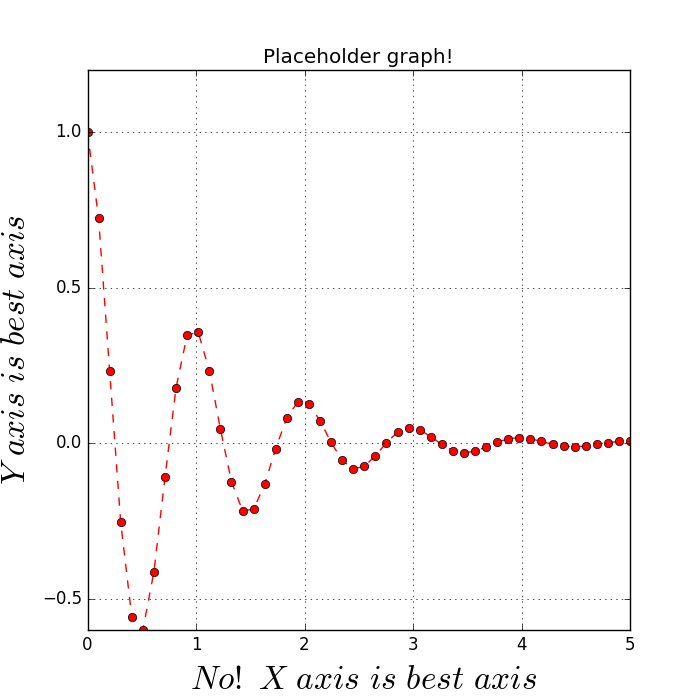
\includegraphics[scale=0.35]{figures/placeholderfig.png}
			\caption{Dynamo Raw Data Histogram (Low Speed)}
			\label{fignoisehistolow}
		\end{subfigure}
		\begin{subfigure}{0.45\textwidth}
			\centering
			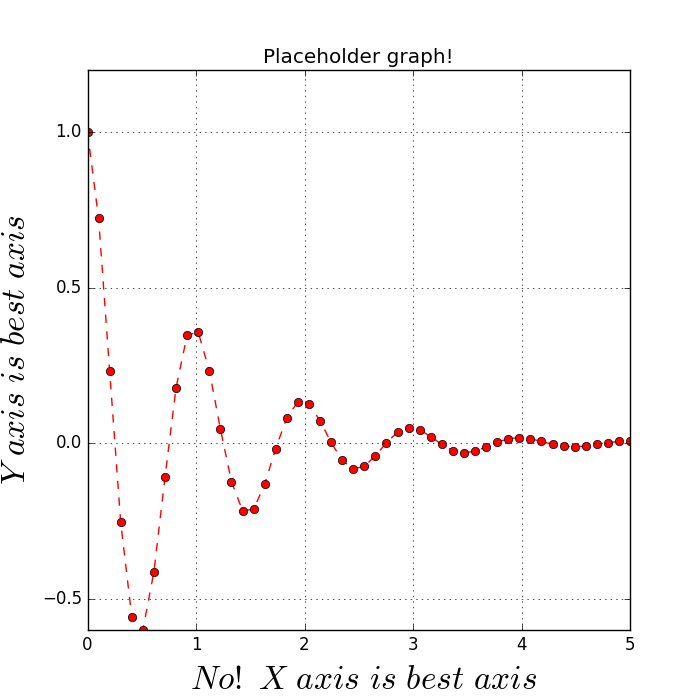
\includegraphics[scale=0.35]{figures/placeholderfig.png}
			\caption{Dynamo Raw Data Histogram (High Speed)}
			\label{fignoisehistohigh}
		\end{subfigure}
	\end{figure}
	
	\subsection*{Current Sensor}
	The sensor was calibrated by reading in from the sensor and comparing this value with the actual current reading obtained using a standard lab multimeter, repeating this at different voltages (thus also different rotational speeds and different currents). An equation was fit to the data (see Figure \ref{figcurevalres}).to give an equation for the current in terms of the HES voltage. A 3$^{rd}$ order equation was found to best fit the experimental results.\br
	Figure \ref{figcurevalres} shows how the calibrated current readings (after filtering) compare with actual values obtained using a multimeter. The values are in agreement, although the data is somewhat noisy despite the applied filtering.
	
	\begin{figure}[!htb]
		\centering
		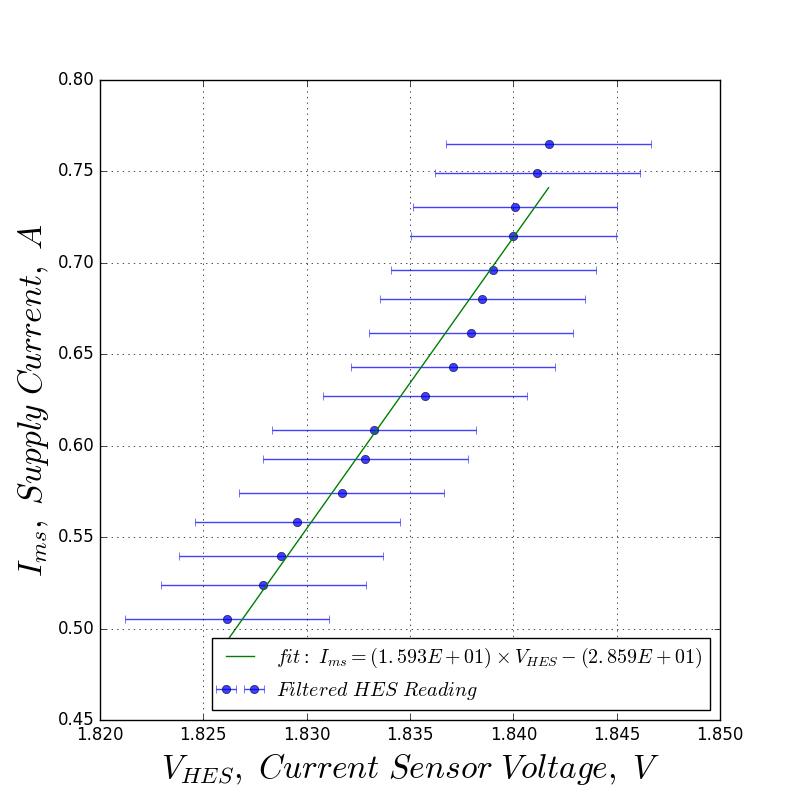
\includegraphics[scale=0.35]{figures/fig_hes_cal.png}
		\caption{Current Sensor Evaluation Results}
		\label{figcurevalres}
		\begin{subfigure}{0.9\textwidth}
			\footnotesize Supply current plotted against the filtered HES input (blue cirles). Error bars represent one standard deviation in the data. A 1$^{st}$ order polynomial was fit to the data (green line).
		\end{subfigure}
	\end{figure}
	
	\subsection*{Data Filtering}
	There were a number of options for data filtering methods to choose from. Each altered the data in different ways. The final chosen method was a Butterworth low-pass frequency filter. The other choices were a gaussian weighted average method, a Wiener filter, and using spline interpolation. Spline interpolation filters the signal by observing the shape of the response and "drawing" a clean signal best suited. It was ruled out for not accurately following the path of the signal. The Gaussian method is a moving average, with the samples weighted according to a Gaussian normal distribution. Gaussian filtering was ruled out as it reacted to slowly to sharp changes in input readings. Wiener filtering uses statistics to estimate the desired output. The Butterworth signal was chosen as the best filter for use in the rheometer as it provided the best tracking of fluctuations in the data whilst eliminating noise. Figure \ref{figfiltcomp} compares the different filtering methods.\\
	
	\begin{figure}[!htb]
		\centering
		\begin{subfigure}[t]{0.22\textwidth}
			\centering
			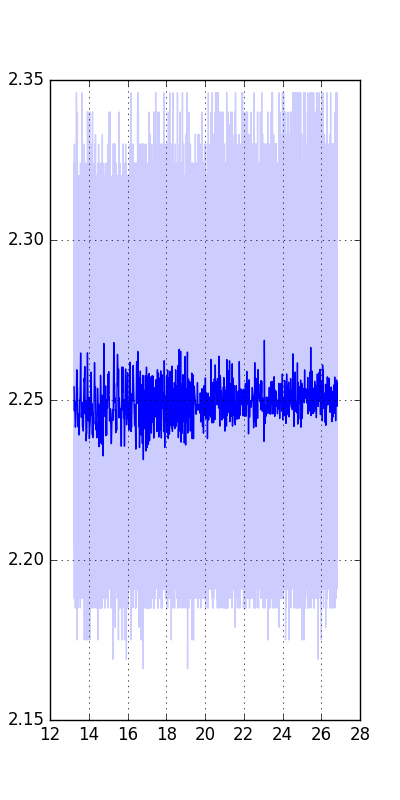
\includegraphics[scale=0.3]{figures/fig_filt_compar_spline.png}
			\caption{Spline Interpolation}
			\label{figfiltsp}
			\footnotesize
		\end{subfigure}
		\begin{subfigure}[t]{0.22\textwidth}
			\centering
			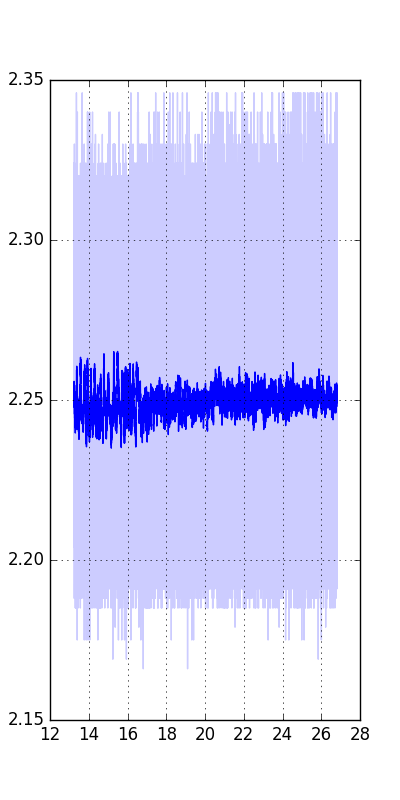
\includegraphics[scale=0.3]{figures/fig_filt_compar_wiener.png}
			\caption{Wiener Filter}
			\label{figfiltwi}
			\footnotesize
		\end{subfigure}
		\begin{subfigure}[t]{0.22\textwidth}
			\centering
			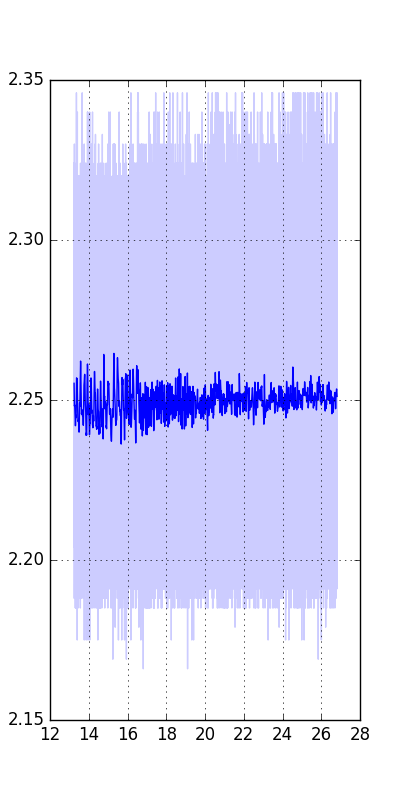
\includegraphics[scale=0.3]{figures/fig_filt_compar_gaussian.png}
			\caption{Gaussian Filter}
			\label{figfiltga}
			\footnotesize
		\end{subfigure}
		\begin{subfigure}[t]{0.22\textwidth}
			\centering
			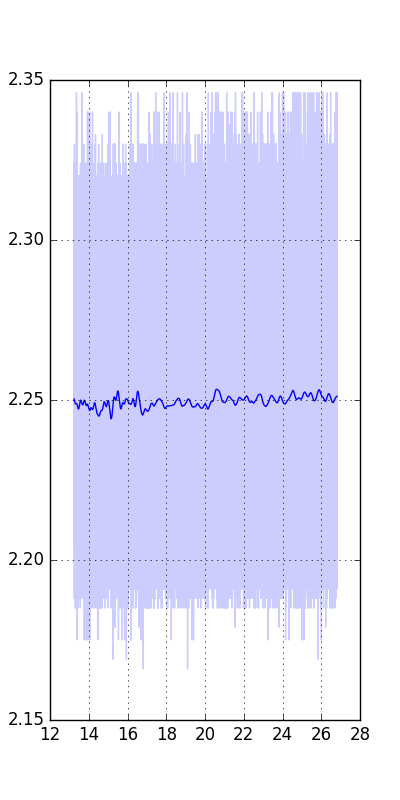
\includegraphics[scale=0.3]{figures/fig_filt_compar_butter.png}
			\caption{Butterworth Filter}
			\label{figfiltbu}
			\footnotesize
		\end{subfigure}
		\caption{Comparison of Filter Methods \label{figfiltcomp}}
	\end{figure}
	
    \noindent
	Due to the Butterworth's nature as a frequency filter, it could cause issue with reading the intermittent jumps up in viscosity due to jamming. This could be circumvented by developing a filter which recognises the different magnitude of jamming to the noise signal. Or the noise could be analysed for constituent signals: the noise could be originating from the 50Hz power supply, or another regular source. Repeated application of different band-stop filters would eliminate the known sources of noise, therefore any remaining disruption in the signal is useful data.

%	\begin{figure}[!htb]
%		{\centering
%			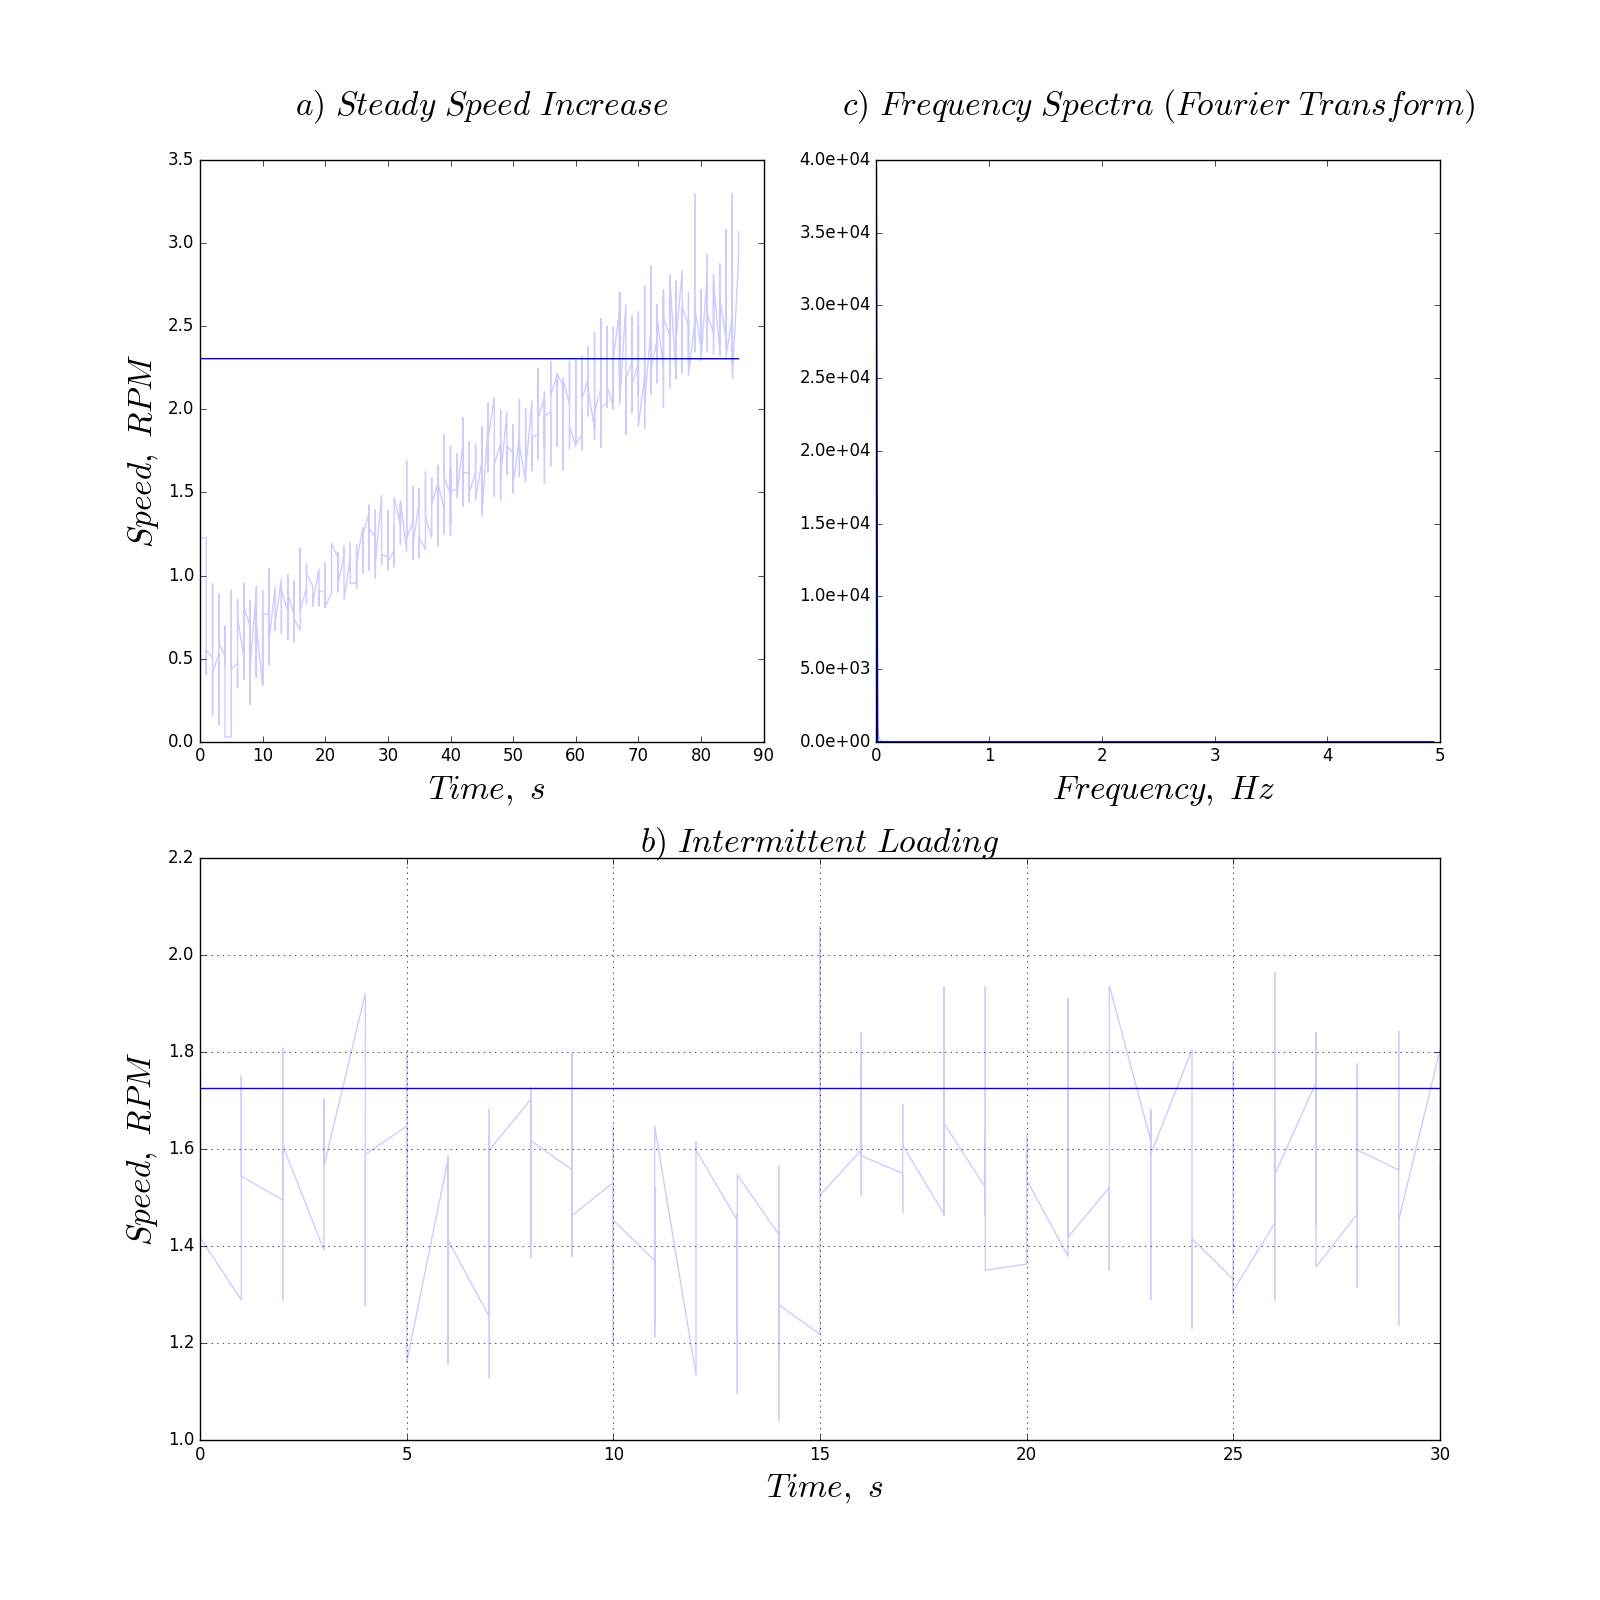
\includegraphics[scale=0.3]{figures/fig_filt_demonstra.png}
%			\caption{Butterworth Filter Demonstration}
%			\label{figfilterdemon}}
%		{\footnotesize Actual data readings (faint blue) were passed through a Butterworth filter to obtain a noise-reduced signal (bright blue).\newline {\bfseries a)} Graph of a steady increase in motor supply voltage, excpeted result is a series of 11 steps.\newline {\bfseries b)} Graph showing speed variance with a random intermittent load applied to the motor (an approximation of a shear thickening fluid)\newline {\bfseries c)} Fourier Transform of the response in b); faint blue line shows the fourier transform of the raw (noisy) data, bright blue shows the filtered response, clearly showing the effect of the filter on the resulting data.}
%	\end{figure}

	\subsection*{Rheometry}
	The rheometer's ability to accurately report the viscosity of a test fluid was evaluated by using the rheometer to measure the viscosity of reference fluids of known viscosity. The results were then compared to the viscosity measurement taken using a standard lab rheometer. The rheometer was used to measure the viscosity of several reference fluids. The rheometer was calibrated with aqueous glycerol solutions (see Table \ref{tabreffluvisc}), before verifying the calibrations by calculating the viscosity of the reference fluids from logged data.
	\br
	The scissor lift was lowered, allowing the rheometer to easily be loaded. The outer cylinder of the rheometer was loaded with 15ml of the first fluid using a 5ml syringe (taking care to avoid bubbles). The scissor lift was then raised into the working position; the two cylinders as close together as possible without them touching. The cylinders were then aligned by turning on the motor and observing the flow of the fluid. The fluid would climb up the side of the cylinder if the inner cylinder was too close. This method of aligning the cylinders was found to be the most accurate and efficient way. On the Raspberry Pi a script was written which will load the motor class, with the appropriate settings, and log data sufficient to calculate the viscosity of the fluid in the rheometer. The script also dictates how the speed of the motor should vary, if at all. The motor's speed (and therefore the rate of strain experienced by the fluid) was kept constant for 5 minutes. This was repeated for each of the four reference solutions, and both pure glycerol and water. The rheometer was calibrated, and then this calibration (together with the other empirical calibrations found previously) was verified by calculating the viscosity of the reference fluids. The results were compared with the results obtained from the DHR-2, as plotted on Figure \ref{figrheotestres}.
	
	\nomenclature[g]{$\mu_{glycerol}$}{Viscosity of glycerol\hfill $Pa.s$}
	\nomenclature[g]{$\mu_{water}$}{Viscosity of water\hfill $Pa.s$}

	\noindent
	\begin{figure}[!htb]
		\centering
		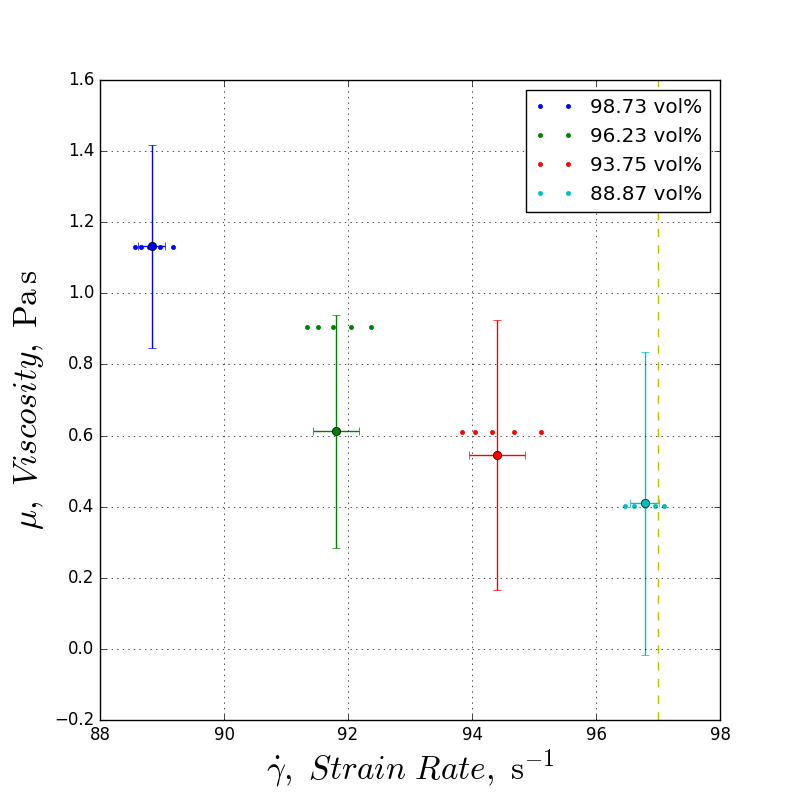
\includegraphics[scale=0.45]{figures/fig_t_ref_check.png}
		\caption{Torque Calibration Check}
		\label{figrheotestres}
		\begin{subfigure}{0.9\textwidth}
			\footnotesize Viscosity of reference fluids plotted against time. Each colour represents a different composition of reference solution (blue - 98.73v\%, green - 96.23v\%, red - 93.75v\%, and cyan - 88.87v\%). The large circles represent the average calculated viscosity for each fluid, the error bars represent one standard deviation. The small circles are the expected viscosities for each of the solutions. The yellow dashed line shows the set strain rate for each of the solutions.
		\end{subfigure}
	\end{figure}

	\subsection*{Control}
	The control system was tested by writing a script to read in the motor's speed, which was converted into a control action using the control class which was applied to the digital potentiometer. This was repeated every 0.1s for 5 minutes. The motor class was used in the script to read the motor's speed, and to set the new supply voltage. The script was extended to log information (potentiometer value, speed, current, control action) about the process' response to a change in set point and amongst disturbances.
	\br
	Before the controller could be used, it needed to be tuned. The tuning was obtained by first introducing a step change in the supply voltage to gauge how the speed (controller input) is affected by the potentiometer value (controller output). The resulting data was plotted (Figure \ref{figsteptest}). A First Order Plus Dead Time (FOPDT) transfer function model was used to model the controller's response under different tunings, the optimal tuning settings found simply by trial and error. The testing script was run with this optimal tuning, the resulting response plotted on Figure \ref{figcontrtest}.
	
	\begin{figure}[!htb]
		\centering
		\begin{subfigure}{0.45\textwidth}
			\centering
			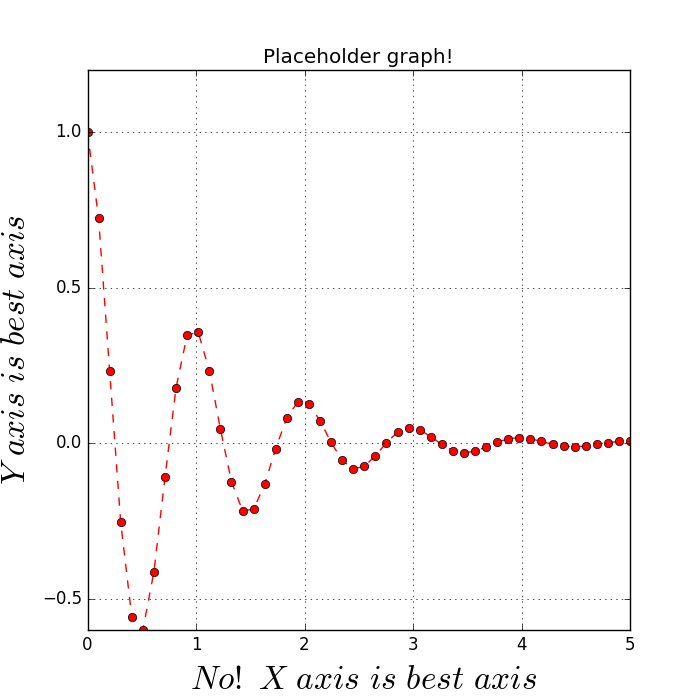
\includegraphics[scale=0.45]{figures/placeholderfig.png}
			\caption{Process Step Test}
			\label{figsteptest}
			\footnotesize 
		\end{subfigure}
		\begin{subfigure}{0.45\textwidth}
			\centering
			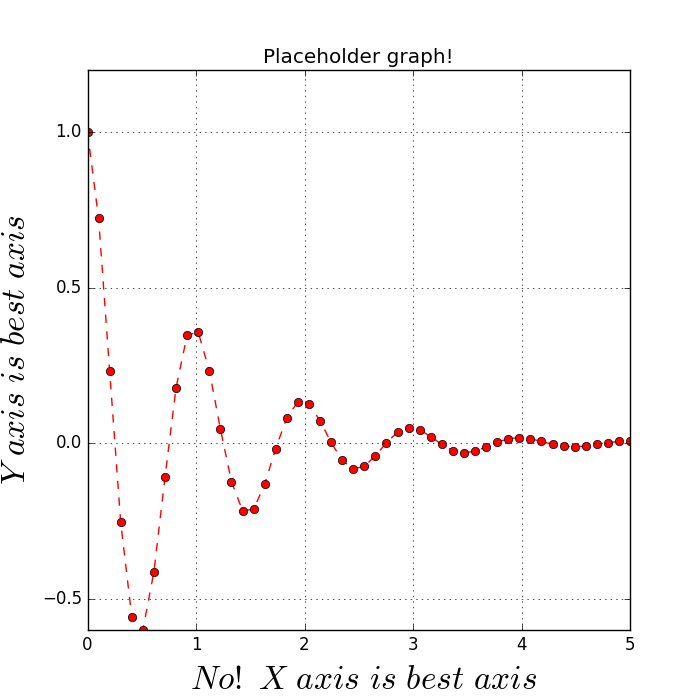
\includegraphics[scale=0.45]{figures/placeholderfig.png}
			\caption{Controller Test}
			\label{figcontrtest}
			\footnotesize 
		\end{subfigure}
	\end{figure}
	
	\noindent
	discussion of results, why wasn't included, 200 words \cbh \cbh \cbh \cbh \br
	There is a clear need for the control system. Looking at Figure \ref{figrheotestres}, it can be seen that the different fluids are sheared at different rates due to their different viscosities. If the viscosity is not known (as would be expected for a fluid placed into a rheometer) this drift from the zero viscosity strain rate cannot be predicted. Instead, a control system should be in place to monitor the speed of the motor and maintain it at a set point to ensure that a desired strain rate is maintained.
%=====------++++++=====------++++++=====------++++++=====------++++++=====------++++++=====------++++++=====------++++++=====------++++++=====------++++++=====------++++++=====------++++++=====------++++++=====------++++++=====------++++++=====------++++++=====------++++++

	\nc{Conclusions}
	%Summarise findings and inferences mentioned in the core of the report. Try to be as brief as possible, with concise statements. Include recommendations, where appropriate. 
	The rheometer does not meet its design criteria. The electronics worked well - the motor supply voltage check proved the circuit delivered the expected voltages, the dynamo and Hall effect sensors read the speed and current adequately too. The system's failing lie in the calibrations and calculation assumptions. When calibrating the torque as a function of motor supply current, the resulting linear fit equation is not sufficient to give the torque at different shear rates - further calibration is required. The motor output torque not only varies with the fluid's viscosity, but also the friction of the gearing attached to the motor. As the speed increases, this friction increases. \cbh
	\br
	The motor was not sensitive at all to changes in torque. A large (several orders of magnitude) change in torque represented a tiny change in the current. The motor was a relatively high power model (up to 15v, 20,000RPM) which was geared to reduce speed. The ratio was 16:1, meaning speed was reduced by a factor of 16, but torque output was increased by a factor of 16. Going backwards, this means that a torque requirement increase at the shaft is reduced 16 times at the motor outlet further decreasing its sensitivity to torque. Given that this was an integral part of the design a new (more sensitive) motor should be sought, or a different method of measuring the shear stress experienced by the fluid should be found. This (more sensitive motor) will allow for more accurate torque measurement by allowing the sensors to pick up a bigger range of current supplies.
	\br
	There was a huge amount of noise in the readings which had to be filtered out. The filter used was a low-pass frequency filter. Any high frequency noise was removed. If a jamming event is high frequency, then this filter will remove it along with the noise resulting in a loss of useful data. Alternative filters are available - Gaussian weighted average, spline smoothing, or Wiener probabilistic filter - however these were discounted for reasons stated earlier. A solution would be to identify the sources of noise in the signal, and specifically remove the noise with a band-stop frequency filter while hopefully leaving the important information in the signal. 
	\br
	One possible source of the noise is variance in the mains power supply. Mains electricity is single phase 50Hz AC - it is a single sinusoidal wave varying from +230V to -230V. When this is converted to DC, the signal is first converted to its absolute value, and is then smoothed out. This may not be done perfectly, resulting in a trace of the original sinusoid in the DC signal. This noise will have a frequency of 50Hz. 
	\br
	The voltage reference used by the ADC to convert real world signals into digital signals could vary if not properly regulated. The 3.3V reference used by the ADC comes from the Raspberry Pi's GPIO header and is regulated by the Raspberry Pi and should not, and does not, vary. A voltmeter was attached and the signal was found to stay constant at 3.3V for the duration and is therefore unlikely as a source of noise. 
	\br
	The sensors themselves are potential sources for noise. The dynamo gave off very noisy data. This noise could arise from the way the dynamo is constructed: a series of coils which, when rotated in a magnetic field, produce a voltage. Since the magnetic field produced by the permanent magnets in the motor is not continuous and homogeneous, the output is going to vary as the motor rotates. Therefore the signal will dip and rise at a frequency of some multiple of the rotation rate. This noise can be reduced by calculating exactly what multiple of the rotation rate (the number of coils in the armature) and also knowing the shape of the noise waveform. Alternatively, other speed measurement methods could be sought. 
	\br % FUTURE WORK
	There is a lot of work that could be done to this system. Future work includes changing out the motor for a motor torque-sensitive model, introducing a piezo-electric stress sensor, and adding a camera for detecting optical evidence of jamming. Piezo electrics are often used as strain sensors in bridges and other systems. Previous work has used the strain sensor as a purely qualitative way of examining jamming (\cite{thescforsyth}). By relating the force observed on the piezo sensor to the drag coefficient of the sensor in the flowing fluid, and therefore the fluid's Reynold's number, the viscosity can be related to the voltage output of the piezo electric device. 
	\br
	Another future step to take with the project would be to use the control system developed along with the addition of some current control circuit to be able to control the shear stress (by controlling the motor torque). This would increase the utility of the rheometer by adding a second operational mode with controlled/constant shear stress as opposed to constant shear rate as it is at the moment.
	
%=====------++++++=====------++++++=====------++++++=====------++++++=====------++++++=====------++++++=====------++++++=====------++++++=====------++++++=====------++++++=====------++++++=====------++++++=====------++++++=====------++++++=====------++++++=====------++++++

%% APPENDIX %%

	\nc{Reflection and Review}
	%lit review, history
	%Relate this section to the learning objectives in the introduction. Report what you have learnt about the organisation and about yourself. Mention your achievements, what you have learnt, skills you have acquired or improved. This might be technical or "soft" skills. Try to relate this to what you have learned in your coursework at University and what skills you will take forward to your first full time professional post.
	The goal of this project was to design, build, and test a rheometer using a Raspberry Pi and open source software.\br
	Over the course of the project I have learned a lot. Working with the Raspberry Pi has taught me a lot about how computers work, how they communicate, and how they may be used in industrial processes. Data processing and storage has been an important concern; with the Raspberry Pi taking thousands of measurements every second. The Pi only has limited memory available, which can fill up quickly. This was circumvented by saving the data to file, rather than keeping it in memory. \br
	Another thing I gained a lot of experience with was data processing. Data recorded from sensors was noisy - due to random fluctuations in temperature, air pressure, vibrations, power supply. The noise was reduced using a filtering algorithm. As I was researching noise filtering I learned about the types of filters and how they work, I learned about how different signal domains (like the frequency domain) can be used to remove unwanted parts of the signal.\br
	[Unfinished section]
	
	

%=====------++++++=====------++++++=====------++++++=====------++++++=====------++++++=====------++++++=====------++++++=====------++++++=====------++++++=====------++++++=====------++++++=====------++++++=====------++++++=====------++++++=====------++++++=====------++++++
	\newpage
	\stepcounter{chapter}
	\addcontentsline{toc}{chapter}{\arabic{chapter} Nomenclature}
	\def\achapter{\arabic{chapter} Nomenclature}
	%List all the symbols in alphabetical order, with Greek symbols at the end
	\printnomenclature[1.5cm]
	
%=====------++++++=====------++++++=====------++++++=====------++++++=====------++++++=====------++++++=====------++++++=====------++++++=====------++++++=====------++++++=====------++++++=====------++++++=====------++++++=====------++++++=====------++++++=====------++++++
	%Main Bibliography
	\newpage
	\addcontentsline{toc}{chapter}{Bibliography}
	\def\achapter{Bibliography}
	%\bibliographystyle{unsrt}
	\bibliographystyle{abbrv}
	\bibliography{biblio}




\appendix


\chapter*{Appendices}
%appendix preamble

\addcontentsline{toc}{chapter}{Appendices}
\def\achapter{Appendices}
\pagenumbering{alph}
\setcounter{page}{1}
\setcounter{secnumdepth}{0}
\setcounter{section}{1}

\newcounter{apsec}
\setcounter{apsec}{0}
\newcounter{apsubsec}
\def\apsect#1{
	\addtocounter{apsec}{1}
	\section{\arabic{apsec}\hskip0.5cm #1}
	\setcounter{apsubsec}{1}
}
\def\apsubsect#1{
	\subsection*{\arabic{apsec}\Alph{apsubsec} \hskip0.5cm #1}
	\addtocounter{apsubsec}{1}
}

\apsect{Source Code}
%-=-=-=-=-=-=-=-=-=-=-=-=-=-=-=-=-=-=-=-=-=-=-=-=-=-=-=-=-=-=-=-=-=-=-=-=-=-=-=-=-=-=-=-=-=-=-=-=-=-=-=-=-=-=-=-=-=-=-=-=-=--=-=-=-=-=-=-=-=-=-=-=-=-=-=-=-=-=-=-=-=-=-=-=-=-=-=-=-=-=-=-=-=-=-=-=-=-=-=-=-=-=-=-=-=-=-=-=-=-=-=-=-=-=-=-=-=-=-=-=-=-=-=-=-=-=-=-=-=-=-=-=-=
As mentioned previously, the software was split up into different sections. This was to make the code more manageable, and easier to maintain. The source code for each class section, as well as the filtering library, is included here.
\apsubsect{ADC Class}
%-=-=-=-=-=-=-=-=-=-=-=-=-=-=-=-=-=-=-=-=-=-=-=-=-=-=-=-=-=-=-=-=-=-=-=-=-=-=-=-=-=-=-=-=-=-=-=-=-=-=-=-=-=-=-=-=-=-=-=-=-=--=-=-=-=-=-=-=-=-=-=-=-=-=-=-=-=-=-=-=-=-=-=-=-=-=-=-=-=-=-=-=-=-=-=-=-=-=-=-=-=-=-=-=-=-=-=-=-=-=-=-=-=-=-=-=-=-=-=-=-=-=-=-=-=-=-=-=-=-=-=-=-=

\begin{Verbatim}[frame=single]
#
# adc.py
#
# Class library, gives support for using the MCP3008 8-channel 10bit ADC
#

import RPi.GPIO as gpio
import spidev as spi


class MCP3008(object):

	bus = 0     # holds the bus connection
	cs_pin = 0  # GPIO pin used to select the chip (gpio.BOARD numbering) 
	            # OR which cs channel to use
	vref = 3.3  # Reference voltage in use
	
	def __init__(self, cs_pin=1, vref=3.3):
		''' 
		object = adc.MCP3008(**kwargs)
		
		Initialise MCP3008 ADC class object.
		
		kwargs:
		cs_pin - SPI chip select. Default is 1.
		vref - ADC reference voltage. Default is 3.3.
		'''
		
		# Chip select setup
		self.cs_pin = cs_pin
		if (cs_pin > 1):  # using the GPIO pins as chip_select pins
			gpio.setmode(gpio.BOARD)
			# chip select is normally high, pulled up by the RPi
			gpio.setup(self.cs_pin, gpio.OUT, pull_up_down=gpio.PUD_UP)  
			gpio.output(self.cs_pin, gpio.HIGH)
		else:  # using the Pi's built in chip select method
			pass
		
		# Set up bus connection
		self.bus = spi.SpiDev()
		
		# Vref setting
		self.vref = vref
	
	def read_data(self, channel):
		'''
		read_data(channel)
		
		Converts the voltage (relative to vref) on the specified channel 
		to a 10-bit number.
		
		channel - (int, 0-7) the ADC data channel that is to be read from.
		
		returns: (int, 0-1023) 10-bit value representing the voltage level 
		         on the channel specified.
		'''
		
		self.open()
		indat = self.bus.xfer2([1, 8 + channel << 4, 0])
		self.close()
		return ((indat[1] & 3) << 8) + indat[2]
	
	def read_volts(self, channel):
		'''
		read_volts(channel)
		
		Reads the voltage level on the specified channel.
		
		channel - (int, 0-7) the ADC data channel that is to be read from.
		
		returns: float representing the voltage level on the channel 
		         specified.
		'''
		
		dat = self.read_data(channel)
		volts = (float(dat) / 1024.0) * self.vref
		return volts
	
	def write_byte(self, byte):
		'''
		write_byte(byte)
		
		byte - the 8 bit command to be sent to the ADC.
		'''
		
		self.open()
		command = [byte, 0]  # Two bytes; first is command shifted 4 bits
		                     # second is zero
		self.bus.writebytes(command)
		self.close()
	
	def open(self):
		'''
		open()
		
		opens a channel to the SPI device.
		
		Must completed by a following close() call.
		'''
		
		if (self.cs_pin > 1):
			gpio.output(self.cs_pin, gpio.HIGH)
			self.bus.open(0, 1)
			self.bus.max_speed_hz = 10000000
		else:
			self.bus.open(0, self.cs_pin)
			self.bus.max_speed_hz = 10000000
	
	def close(self):
		'''
		close()
		
		closes a (previously opened) channel to the SPI device.
		'''
		
		if (self.cs_pin > 1):
			gpio.output(self.cs_pin, gpio.LOW)
			self.bus.close()
		else:
			self.bus.close()
\end{Verbatim}
\apsubsect{Digital Potentiometer Class}
%-=-=-=-=-=-=-=-=-=-=-=-=-=-=-=-=-=-=-=-=-=-=-=-=-=-=-=-=-=-=-=-=-=-=-=-=-=-=-=-=-=-=-=-=-=-=-=-=-=-=-=-=-=-=-=-=-=-=-=-=-=--=-=-=-=-=-=-=-=-=-=-=-=-=-=-=-=-=-=-=-=-=-=-=-=-=-=-=-=-=-=-=-=-=-=-=-=-=-=-=-=-=-=-=-=-=-=-=-=-=-=-=-=-=-=-=-=-=-=-=-=-=-=-=-=-=-=-=-=-=-=-=-=
\begin{Verbatim}[frame=single]
#
# dig_pot.py
#
# provides support for using an MCP4131 digital potentiometer with the raspberry pi

import spidev as spi

class MCP4131(object):
	'''
	SPI 10K Digital Potentiometer
	'''
	bus = 0  # holds the bus connection to the digital pot
	lav = 0
	chip_select = 0
	
	def __init__(self, chipselect=0):
		'''
		MCP4131()
		
		Creates an instance of the MCP4131 class for communicating over SPI 
		with an MCP4131 digital potentiometer.
		
		kwargs:
		chipselect -  the chip_select address for the MCP4131 chip on the 
		              SPI network.
		'''
		self.bus = spi.SpiDev()
		self.chip_select = chipselect
	
	def set_resistance(self, value):
		'''
		set_resistance(value)
		Sets the value on the potentiometer.
		
		value - integer value to set on the potentiometer. The resistance 
		        betweeen the A terminal and the wiper will vary directly 
		        with this value.
		'''
		self.lav = value
		self.write_byte(value)
	
	def write_byte(self, byte):
		'''
		write_byte(byte)
		
		Writes the specified byte to the digital potentiometer.
		
		byte - the value to send to the potentiometer.
		'''
		self.open()
		command = [0, byte]
		self.bus.writebytes(command)
		self.close()
	
	def open(self):
		'''
		open()
		
		Begins communication with the potentiometer.
		Must be matched by an accompanying "close()"
		'''
		self.bus.open(0, self.chip_select)
		self.bus.max_speed_hz = 10000000
	
	def close(self):
		'''
		close()
		
		Ends communication with the potentiometer.
		'''
		self.bus.close()
\end{Verbatim}
\apsubsect{Motor Class}
%-=-=-=-=-=-=-=-=-=-=-=-=-=-=-=-=-=-=-=-=-=-=-=-=-=-=-=-=-=-=-=-=-=-=-=-=-=-=-=-=-=-=-=-=-=-=-=-=-=-=-=-=-=-=-=-=-=-=-=-=-=--=-=-=-=-=-=-=-=-=-=-=-=-=-=-=-=-=-=-=-=-=-=-=-=-=-=-=-=-=-=-=-=-=-=-=-=-=-=-=-=-=-=-=-=-=-=-=-=-=-=-=-=-=-=-=-=-=-=-=-=-=-=-=-=-=-=-=-=-=-=-=-=
\begin{Verbatim}[frame=single]
INSERT_FROM("./../bin/motor.py")
\end{Verbatim}
\apsubsect{Controller class}
%-=-=-=-=-=-=-=-=-=-=-=-=-=-=-=-=-=-=-=-=-=-=-=-=-=-=-=-=-=-=-=-=-=-=-=-=-=-=-=-=-=-=-=-=-=-=-=-=-=-=-=-=-=-=-=-=-=-=-=-=-=--=-=-=-=-=-=-=-=-=-=-=-=-=-=-=-=-=-=-=-=-=-=-=-=-=-=-=-=-=-=-=-=-=-=-=-=-=-=-=-=-=-=-=-=-=-=-=-=-=-=-=-=-=-=-=-=-=-=-=-=-=-=-=-=-=-=-=-=-=-=-=-=
\begin{Verbatim}[frame=single]
INSERT_FROM("./../bin/control.py")
\end{Verbatim}
\apsubsect{Filtering}
%-=-=-=-=-=-=-=-=-=-=-=-=-=-=-=-=-=-=-=-=-=-=-=-=-=-=-=-=-=-=-=-=-=-=-=-=-=-=-=-=-=-=-=-=-=-=-=-=-=-=-=-=-=-=-=-=-=-=-=-=-=--=-=-=-=-=-=-=-=-=-=-=-=-=-=-=-=-=-=-=-=-=-=-=-=-=-=-=-=-=-=-=-=-=-=-=-=-=-=-=-=-=-=-=-=-=-=-=-=-=-=-=-=-=-=-=-=-=-=-=-=-=-=-=-=-=-=-=-=-=-=-=-=
\begin{Verbatim}[frame=single]
INSERT_FROM("./../bin/filter.py")
\end{Verbatim}
\apsect{Alternative Designs}
%-=-=-=-=-=-=-=-=-=-=-=-=-=-=-=-=-=-=-=-=-=-=-=-=-=-=-=-=-=-=-=-=-=-=-=-=-=-=-=-=-=-=-=-=-=-=-=-=-=-=-=-=-=-=-=-=-=-=-=-=-=--=-=-=-=-=-=-=-=-=-=-=-=-=-=-=-=-=-=-=-=-=-=-=-=-=-=-=-=-=-=-=-=-=-=-=-=-=-=-=-=-=-=-=-=-=-=-=-=-=-=-=-=-=-=-=-=-=-=-=-=-=-=-=-=-=-=-=-=-=-=-=-=
\apsubsect{Motor Rotation Rate Measurement}
%-=-=-=-=-=-=-=-=-=-=-=-=-=-=-=-=-=-=-=-=-=-=-=-=-=-=-=-=-=-=-=-=-=-=-=-=-=-=-=-=-=-=-=-=-=-=-=-=-=-=-=-=-=-=-=-=-=-=-=-=-=--=-=-=-=-=-=-=-=-=-=-=-=-=-=-=-=-=-=-=-=-=-=-=-=-=-=-=-=-=-=-=-=-=-=-=-=-=-=-=-=-=-=-=-=-=-=-=-=-=-=-=-=-=-=-=-=-=-=-=-=-=-=-=-=-=-=-=-=-=-=-=-=
\large Hall Effect Sensor \normalsize \br
A Hall Effect Sensor (HES) is a device which reacts to the presence of a magnetic field. There exist packages containing HESs which can be used to detect the presence of a magnetic field and thus output a digital signal based upon this. The rotational speed of the motor could be detected by attaching a magnet to the rotating cylinder and using an HES (model number US5881) to detect when a magnet passes a point. Using this, the time between the magnet detections can be used to calculate the rotation rate of the motor. \br
The Hall Effect Sensor is powered by the Raspberry Pi's 5v line and connected to ground. The output pin will be in a high state (0.6v) until the sensor detects the south pole of a magnet, at which point the output will go low (0v). To communicate with the Raspberry Pi, this signal must be converted into 3.3v logic (either a 3.3v high signal or 0v low signal). To achieve this, GPIO pin 23 on the Raspberry Pi was pulled high (set to a high logic signal) and connected through a transistor to ground. Normally, the high input to the transistor allows the flow of current from the GPIO pin to ground, meaning it has a low value. When the hall effect sensor detects a magnet the high signal to the transistor will block the flow of current between the GPIO pin and ground - the GPIO pin will go high. Figure \ref{circhall} shows the schematic of this circuit. \newline
\begin{figure}[!htb]
	\centering
	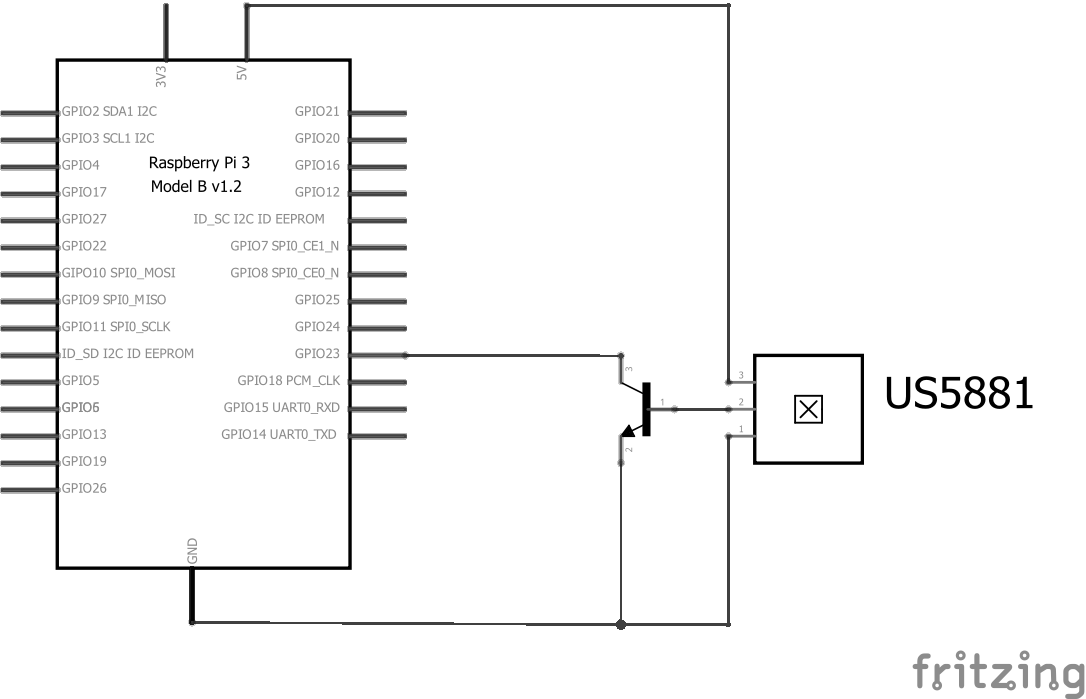
\includegraphics[scale=0.3]{images/circspeeddet.png}
	\caption{Hall Effect Speed Detector Circuit Diagram}
	\label{circhall}
\end{figure} \newline  \noindent
This circuit does not measure the instantaneous rotational speed of the motor. Instead it measures the average speed. By using more magnets, and a smaller time-frame, the speed measured becomes closer to an instantaneous speed. The advantage of using this circuit is that it is simple to set up and use, other speed detection circuits require the use of lasers and photodiodes/phototransistors, or dc dynamos and analogue to digital converters. However, the main downside lies in having to attach magnets at regular intervals to the rotating cylinder, which will have to be done accurately. Another downside is the range of the hall effect sensor. The sensor must be within 10mm of the magnet for it to be able recognise it. \newline \newline \noindent
\large Light Sensor \normalsize \br
The rotational speed of the motor was measured using a light-gate type set up. An IR-LED and IR-phototransistor were set up near the inner cylinder. A metal trip was attached to the cylinder such that it broke the light beam between the LED and the phototransistor. The transistor was set up as a switch such that when light was allowed to fall onto the transistor, a complete circuit was made between GPIO23 (pulled high by the build in resistor) and ground on the Raspberry pi, thus a low value is read. When the beam is broken, this circuit breaks too, causing the value of GPIO23 to go high. On the software side, this value change can be detected and the timing of which can be used to calculate the speed. \newline

\apsect{Further Information} %-=-=-=-=-=-=-=-=-=-=-=-=-=-=-=-=-=-=-=-=-=-=-=-=-=-=-=-=-=-=-=-=-=-=-=-=-=-=-=-=-=-=-=-=-=-=-=-=-=-=-=-=-=-=-=-=-=-=-=-=-=--=-=-=-=-=-=-=-=-=-=-=-=-=-=-=-=-=-=-=-=-=-=-=-=-=-=-=-=-=-=-=-=-=-=-=-=-=-=-=-=-=-=-=-=-=-=-=-=-=-=-=-=-=-=-=-=-=-=-=-=-=-=-=-=-=-=-=-=-=-=-=-=
\apsubsect{Signal Filtering}%-=-=-=-=-=-=-=-=-=-=-=-=-=-=-=-=-=-=-=-=-=-=-=-=-=-=-=-=-=-=-=-=-=-=-=-=-=-=-=-=-=-=-=-=-=-=-=-=-=-=-=-=-=-=-=-=-=-=-=-=-=--=-=-=-=-=-=-=-=-=-=-=-=-=-=-=-=-=-=-=-=-=-=-=-=-=-=-=-=-=-=-=-=-=-=-=-=-=-=-=-=-=-=-=-=-=-=-=-=-=-=-=-=-=-=-=-=-=-=-=-=-=-=-=-=-=-=-=-=-=-=-=-=
Analogue readings of real world data can be corrupted by noise. Noise can appear due to fluctuations in atmospheric conditions, electrical supply, or thermodynamic fluctuation in the reading material (to name a few). For the data to be useful, there must be some provision for reducing the noise. Signal filters can be used to reduce the amount of noise, these can be hardware or software filters. Both represent the same concepts, but in different implementations. Hardware implementation is in continuous time, while software uses discrete time approximations of the same models and functions as hardare filtering. Discussed here are software filtering techniques. \br

% notes -->>
% transform based signal processing methods
%	"express a signal in terms of a combination of a set of elementary signals [... that can be easily analysed]"
% source-filter model based signal processing
%	use a model to obtain the true form of the signal - expressing the predictable structures of the signal, expected patterns.
%	sensitive to deviations from the model
%	used in voice recognition, telephony, video encoding, high-res spectral analysis
% bayesian statistical model based signal processing
%	uses cost-weighted (bayesian philosophical) probability to obtain a model of the "statistical average" values
% neural networks XX
% <<-- notes from wileyadvsignproc.pdf

% from messing around, butterworth seems to give the best representation of the data as noiselessly and as correct as possible.

%Appendix Bibliography

\end{document}